%==== KNITR ===================================================================%



%==== START ===================================================================%

\documentclass[10pt]{beamer}\usepackage[]{graphicx}\usepackage[table]{xcolor}
% maxwidth is the original width if it is less than linewidth
% otherwise use linewidth (to make sure the graphics do not exceed the margin)
\makeatletter
\def\maxwidth{ %
  \ifdim\Gin@nat@width>\linewidth
    \linewidth
  \else
    \Gin@nat@width
  \fi
}
\makeatother

\definecolor{fgcolor}{rgb}{0.345, 0.345, 0.345}
\newcommand{\hlnum}[1]{\textcolor[rgb]{0.686,0.059,0.569}{#1}}%
\newcommand{\hlsng}[1]{\textcolor[rgb]{0.192,0.494,0.8}{#1}}%
\newcommand{\hlcom}[1]{\textcolor[rgb]{0.678,0.584,0.686}{\textit{#1}}}%
\newcommand{\hlopt}[1]{\textcolor[rgb]{0,0,0}{#1}}%
\newcommand{\hldef}[1]{\textcolor[rgb]{0.345,0.345,0.345}{#1}}%
\newcommand{\hlkwa}[1]{\textcolor[rgb]{0.161,0.373,0.58}{\textbf{#1}}}%
\newcommand{\hlkwb}[1]{\textcolor[rgb]{0.69,0.353,0.396}{#1}}%
\newcommand{\hlkwc}[1]{\textcolor[rgb]{0.333,0.667,0.333}{#1}}%
\newcommand{\hlkwd}[1]{\textcolor[rgb]{0.737,0.353,0.396}{\textbf{#1}}}%
\let\hlipl\hlkwb

\usepackage{framed}
\makeatletter
\newenvironment{kframe}{%
 \def\at@end@of@kframe{}%
 \ifinner\ifhmode%
  \def\at@end@of@kframe{\end{minipage}}%
  \begin{minipage}{\columnwidth}%
 \fi\fi%
 \def\FrameCommand##1{\hskip\@totalleftmargin \hskip-\fboxsep
 \colorbox{shadecolor}{##1}\hskip-\fboxsep
     % There is no \\@totalrightmargin, so:
     \hskip-\linewidth \hskip-\@totalleftmargin \hskip\columnwidth}%
 \MakeFramed {\advance\hsize-\width
   \@totalleftmargin\z@ \linewidth\hsize
   \@setminipage}}%
 {\par\unskip\endMakeFramed%
 \at@end@of@kframe}
\makeatother

\definecolor{shadecolor}{rgb}{.97, .97, .97}
\definecolor{messagecolor}{rgb}{0, 0, 0}
\definecolor{warningcolor}{rgb}{1, 0, 1}
\definecolor{errorcolor}{rgb}{1, 0, 0}
\newenvironment{knitrout}{}{} % an empty environment to be redefined in TeX

\usepackage{alltt}

% --- THEME SETUP ---
\usetheme{Madrid}
\usecolortheme{beaver}

% --- PACKAGES ---
\usepackage[utf8]{inputenc}
\usepackage{amsmath,amssymb}
\usepackage{graphicx}
\usepackage{booktabs}
\usepackage{hyperref}
\usepackage{natbib}
\setcitestyle{authoryear,open={(},close={)}}
\usepackage[table]{xcolor}
\usepackage{caption}

% --- CUSTOM COLOR & FONT OVERRIDES ---
\definecolor{beaverRed}{RGB}{140,45,45}
\definecolor{MainColour}{RGB}{0,72,144}
\definecolor{grey}{RGB}{216,221,227}
\definecolor{darkgrey}{RGB}{149,153,158}

\setbeamercolor{title}{bg=MainColour, fg=white}
\setbeamercolor{frametitle}{bg=MainColour, fg=white}
\setbeamercolor{subtitle}{fg=white}
\setbeamercolor{date in head/foot}{bg=MainColour, fg=white}
\setbeamercolor{footline}{bg=MainColour, fg=white}
\setbeamercolor{block title alerted}{bg=MainColour, fg=white}
\setbeamercolor{block body alerted}{bg=grey, fg=black}
\setbeamercolor{block title}{bg=darkgrey, fg=white}
\setbeamercolor{block body}{bg=grey, fg=black}

\setbeamertemplate{caption}[numbered]

\setbeamertemplate{footline}{%
  \leavevmode%
  \hbox{%
    \begin{beamercolorbox}[wd=6.4cm,ht=2.25ex,dp=1ex,leftskip=0.5cm]{date in head/foot}%
      \usebeamerfont{date in head/foot}\insertdate
    \end{beamercolorbox}%
    \begin{beamercolorbox}[wd=6.4cm,ht=2.25ex,dp=1ex]{date in head/foot}%
      \usebeamerfont{date in head/foot}\hfill\insertframenumber\hspace*{0.75cm}
    \end{beamercolorbox}}%
  \vskip0pt%
}

\setbeamertemplate{navigation symbols}{}

% --- METADATA ---
\title{Factor (stochastic) volatility scaling and its application in portfolio optimization}
\subtitle{Mureira \& Muir (2017) with extensions to multivariate mean-variance optimization}
\author{}
\institute[WU]{Vienna University of Economics and Business \\
        \medskip
        \scriptsize Bayesian Econometrics -- Summer Term 2026}
\date{26th of March, 2026}

%==== Beginning of the document ===============================================%

\IfFileExists{upquote.sty}{\usepackage{upquote}}{}
\begin{document}

%==== Title Page ==============================================================%

\begin{frame}
  \titlepage
\end{frame}

%==== Outline =================================================================%

\begin{frame}{Outline}
  \tableofcontents
\end{frame}

%==== 01 - Research Question ==================================================%

\section{Research Questions}
\begin{frame}{Research Questions}
  \begin{itemize}
    \setlength\itemsep{1.5em}
    \item \textbf{RQ 1:} Does volatility forecasting using Bayesian stochastic volatility models improve upon the Moreira \& Muir (2017) historical realized volatility scaling methodology?
    \item \textbf{RQ 2:} Can this dynamic volatility scaling approach be effectively extended to a multi-asset allocation framework?
  \end{itemize}
\end{frame}

%==== 02 - Model Introduction =================================================%

\section{Model Introduction}
\begin{frame}{Stochastic Volatility in a Multivariate Framework}

  \textbf{Goal:} Model the time-varying covariance matrix $\Sigma_t$ for $m$ assets without estimating $\mathcal{O}(m^2)$ parameters per time step.

  \vspace{0.4em}
  
  \begin{alertblock}{Factor Stochastic Volatility (FSV) Model}
    \[
      \mathbf{y}_t = \boldsymbol{\Lambda} \mathbf{f}_t + \boldsymbol{\varepsilon}_t
    \]
  \end{alertblock}

  \begin{itemize}
    \setlength\itemsep{0.5em}
    \item $\boldsymbol{\Lambda}$ ($m \times r$): Latent factor loadings.
    \item $\mathbf{f}_t \sim \mathcal{N}_r(\mathbf{0}, V_t)$: $r$ latent factors, where $V_t$ contains independent SV processes.
    \item $\boldsymbol{\varepsilon}_t \sim \mathcal{N}_m(\mathbf{0}, U_t)$: Idiosyncratic errors, where $U_t$ contains independent SV processes.
  \end{itemize}

  \vspace{0.2em}
  \begin{block}{Covariance Formula}
    $\Sigma_t = \boldsymbol{\Lambda} V_t \boldsymbol{\Lambda}^\prime + U_t$. This isolates risk into manageable factors, creating a predictive $\Sigma_{t+1}$ using only data up to time $t$.
  \end{block}

\end{frame}

\begin{frame}{FSV Intuition: What Is $\mathbf{y}_t$ and Why Factors?}

  \textbf{Observed data:} $\mathbf{y}_t$ is the vector of demeaned daily returns for all assets at time $t$.

  \vspace{0.4em}
  \begin{alertblock}{Signal decomposition}
    \[
      \mathbf{y}_t=\boldsymbol{\Lambda}\mathbf{f}_t+\boldsymbol{\varepsilon}_t
    \]
  \end{alertblock}

  \begin{itemize}
    \setlength\itemsep{0.6em}
    \item $\mathbf{f}_t$: a few \textbf{common market drivers} (equity/rates/risk appetite) with time-varying volatility.
    \item $\boldsymbol{\varepsilon}_t$: \textbf{asset-specific noise} with its own time-varying volatility.
    \item $\boldsymbol{\Lambda}$ maps each asset to each latent driver, so co-movement is explained by shared factors.
    \item Intuition: instead of estimating every covariance element directly, FSV learns a low-dimensional risk engine and updates it through time.
  \end{itemize}

  \vspace{0.2em}
  \begin{block}{Why this helps volatility scaling}
    We get a forward-looking covariance forecast $\hat{\Sigma}_{t+1|t}$ that reacts to changing regimes and cross-asset linkages, not just past window averages.
  \end{block}

\end{frame}

%==== 03 - Moreira & Muir Summary =============================================%

\section{Moreira \& Muir (2017)}
\begin{frame}{Volatility-Managed Portfolios (Moreira \& Muir, 2017)}

  \begin{itemize}
    \setlength\itemsep{1.0em}
    \item \textbf{Core Insight:} Volatility is highly forecastable, but expected returns are not. When volatility spikes, returns do not increase proportionally to compensate for the risk.
    \item \textbf{Methodology:} Scale portfolio exposure inversely proportional to recent realized variance ($\hat{\sigma}^2_t$).
    \item \textbf{The Scaling Rule:} 
      \[
        w_t = \frac{c}{\hat{\sigma}^2_t}
      \]
      where $c$ is a constant chosen so that the unconditional average managed exposure $\bar{w}$ revolves around 1.
    \item \textbf{Conclusion in Paper:} This strategy yields significant alpha, increases Sharpe ratios, and sidesteps crashes, albeit relying on backwards-looking 22-day rolling realized variance.
  \end{itemize}

\end{frame}

%==== 04 - New Methodology ====================================================%

\section{New Methodology}
\begin{frame}{The Proposed Methodology}

  \textbf{Motivation:} If volatility scaling derives its alpha from the predictability of variance, then using a theoretically sound predictive SV model should outperform a naive rolling-window metric.

  \vspace{0.5em}

  \begin{itemize}
    \setlength\itemsep{0.8em}
    \item \textbf{Single-Asset (SPY):} Keep the Moreira \& Muir scaling rule and only swap the variance input:
      \begin{itemize}
        \item Na\"ive model: past 22-day realised variance
        \item FSV model: 22-day horizon-average forecast variance
      \end{itemize}
    \item \textbf{Multi-Asset Framework:} 
      \begin{itemize}
        \item Predict covariance using either rolling 22-day sample covariance or FSV one-step-ahead covariance.
        \item Estimate expected returns ($\hat{\mu}_{t}$) using an expanding mean (causal).
        \item Apply long-only mean-variance allocation within Equities, Bonds, and Gold under fixed budgets (45/45/10 and 60/40/0).
      \end{itemize}
  \end{itemize}

\end{frame}

\begin{frame}{Part 1 Methodology: Exact Weight Construction}

  \textbf{Rebalancing schedule:} every 22 trading days, out-of-sample (test) period only.

  \vspace{0.5em}
  \textbf{Variance inputs at decision time $t$:}
  \[
    \hat{v}^{\text{naive}}_t = \frac{1}{22}\sum_{k=1}^{22} r^2_{t-k}
  \]
  \[
    \hat{v}^{\text{fsv}}_t = \frac{1}{22}\sum_{h=1}^{22}\hat{\Sigma}^{\text{FSV}}_{t+h|t,\text{SPY},\text{SPY}}
  \]

  \vspace{0.5em}
  \textbf{Moreira \& Muir scaling constants (training sample):}
  \[
    c = \left(\frac{1}{N_{\text{train}}}\sum_{t \in \text{train}} \frac{1}{\hat{v}_t}\right)^{-1}
  \]

  \vspace{0.5em}
  \textbf{Managed SPY weights:}
  \[
    w_t = \min\!\left(\max\!\left(\frac{c}{\hat{v}_t},\,0\right),\,w_{\max}\right), \quad w_{\max}=2
  \]
  Benchmark strategy uses $w_t=1$.

\end{frame}


%==== 05 - Results ============================================================%

\section{Results}

%---- 5.1 - Results Overview --------------------------------------------------%

\begin{frame}{Results: Overview}

  \begin{alertblock}{Test Period}
    All results cover \textbf{January 2019 -- December 2024} (out-of-sample).
    The FSV model uses expanding-window refits with \textbf{no look-ahead bias}.
  \end{alertblock}

  \vspace{0.5em}

  \begin{block}{Part 1 \textendash{} Single Asset (SPY)}
    \begin{itemize}
      \setlength\itemsep{0.4em}
      \item FSV volatility scaling \textbf{dominates na\"{i}ve M\&M}: lower realised volatility,
            smaller drawdown, higher return/vol ratio, and \textbf{30\% less turnover}.
      \item Neither scaling strategy beats the buy-and-hold Sharpe during the
            low-volatility, high-momentum 2019--2024 regime.
    \end{itemize}
  \end{block}

\end{frame}

%---- 5.2 - Part 1: Volatility Signal ----------------------------------------%

\begin{frame}{Part 1 -- SPY: Volatility Forecast Quality}

  \begin{figure}
    \centering
    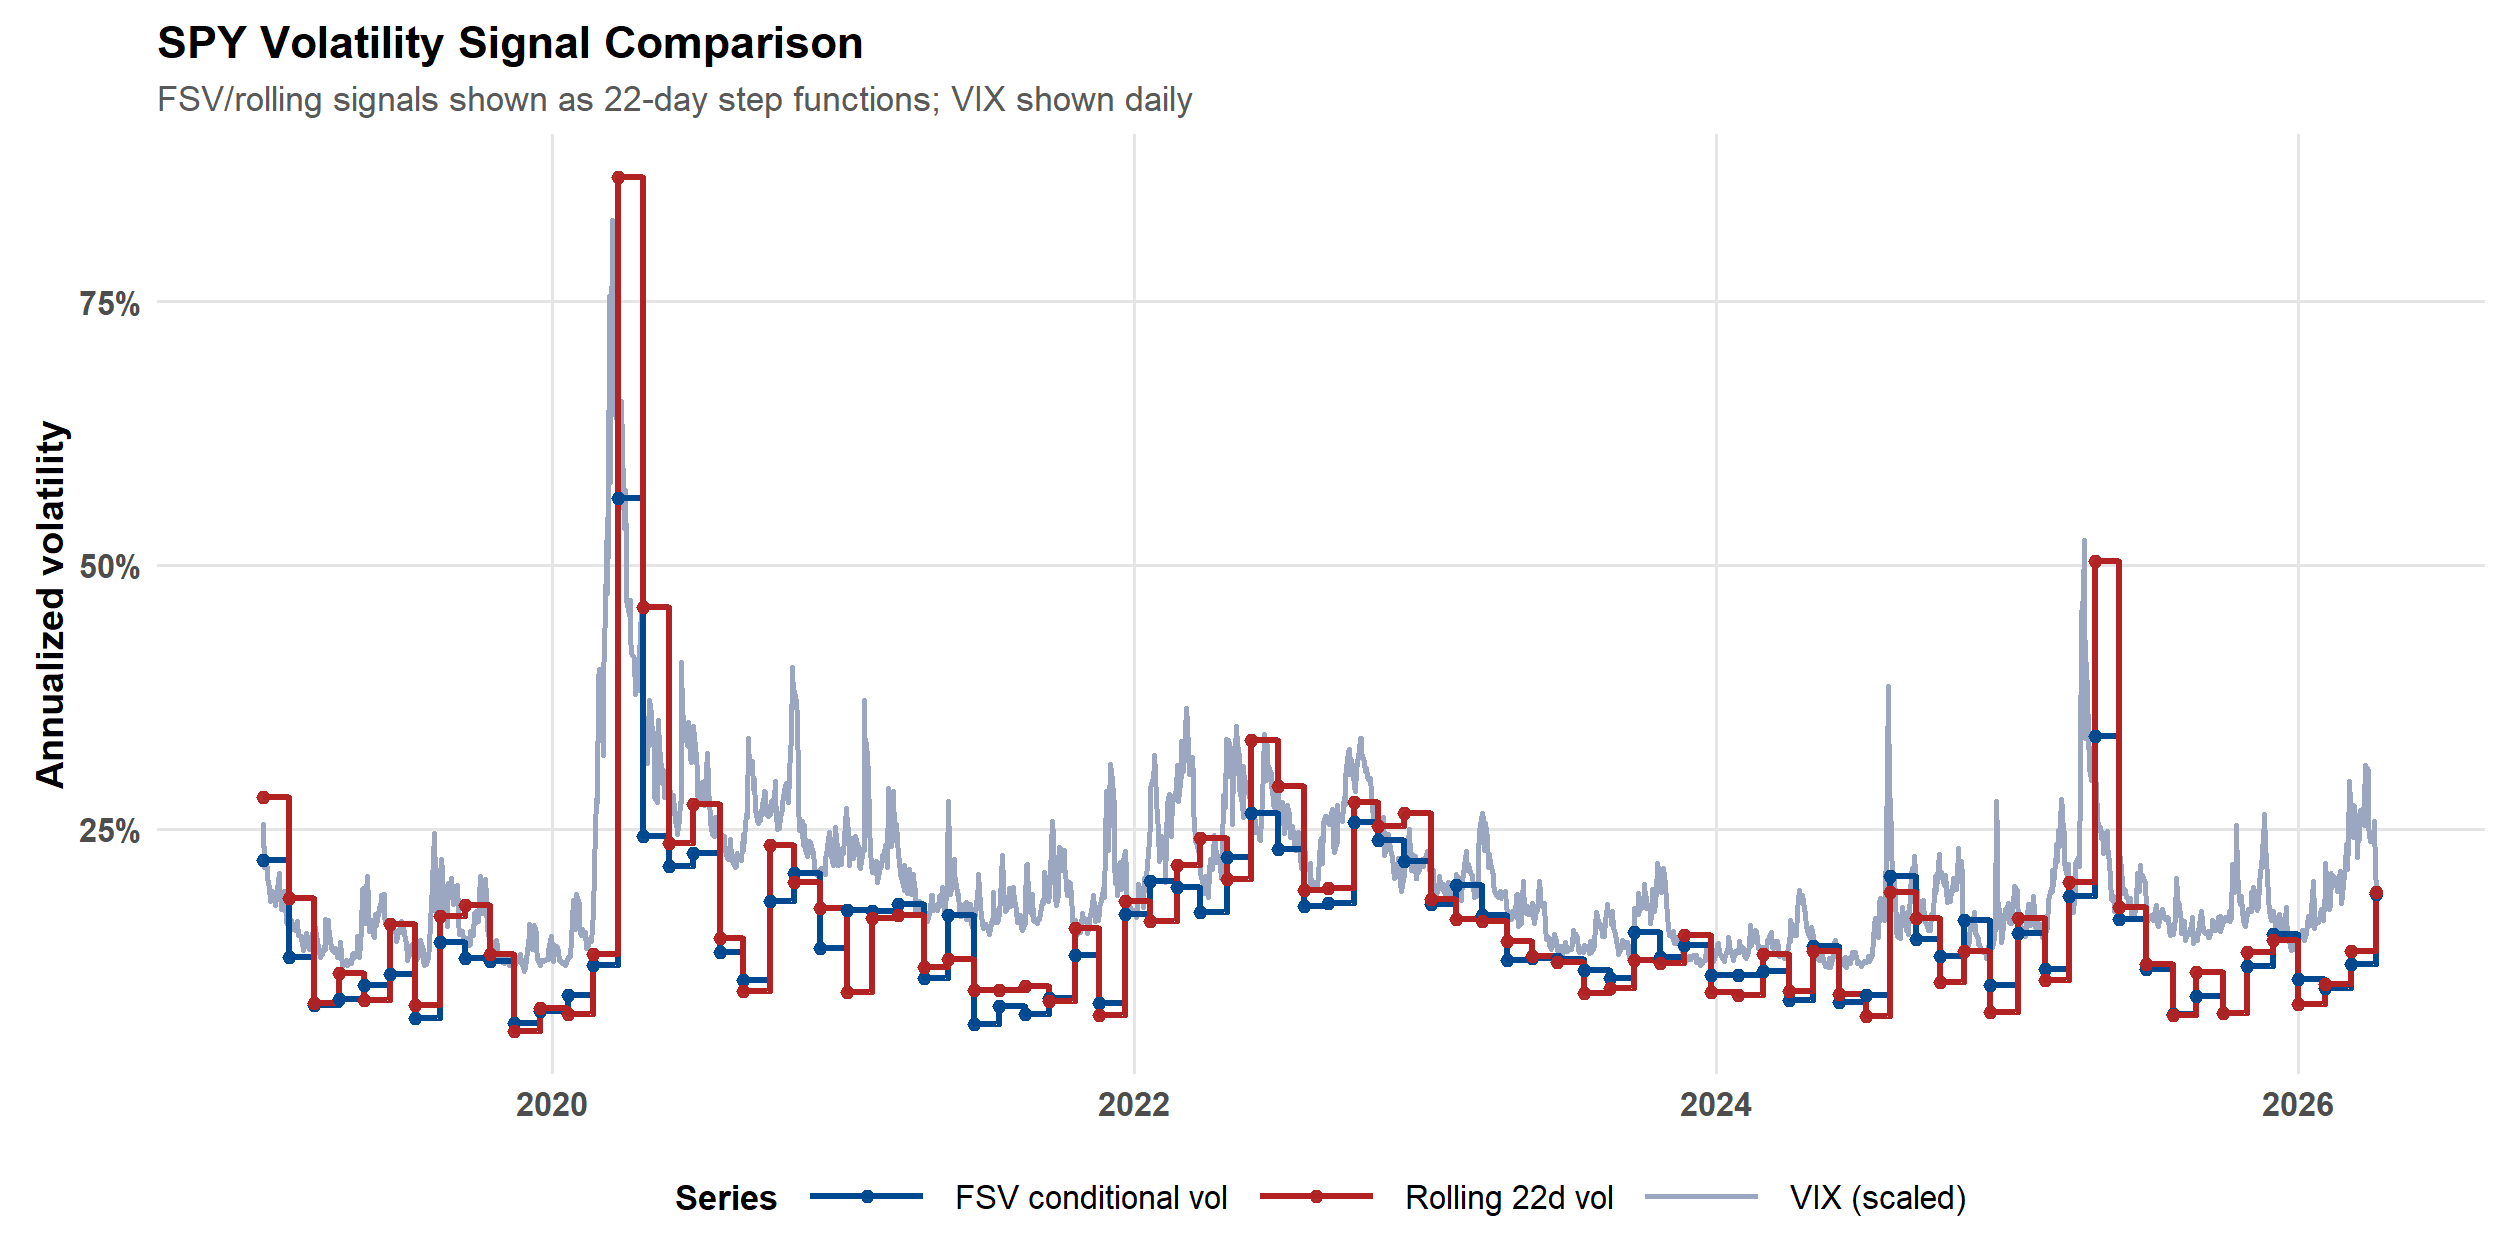
\includegraphics[width=0.92\textwidth]{../03_Results/Charts/part1_spy_vol_vs_vix.png}
    \caption{FSV conditional volatility vs.\ rolling 22-day realised volatility and VIX
             (annualised, test period Jan 2019 -- Dec 2024).
             AR(1) persistence $\hat{\phi} \approx 0.999$.}
  \end{figure}

\end{frame}

%---- 5.25 - Part 1: VIX Pairwise Comparison and Deviation --------------------%

\begin{frame}{Part 1 -- SPY: VIX Pairwise Comparison and Deviation}

  \begin{figure}
    \centering
    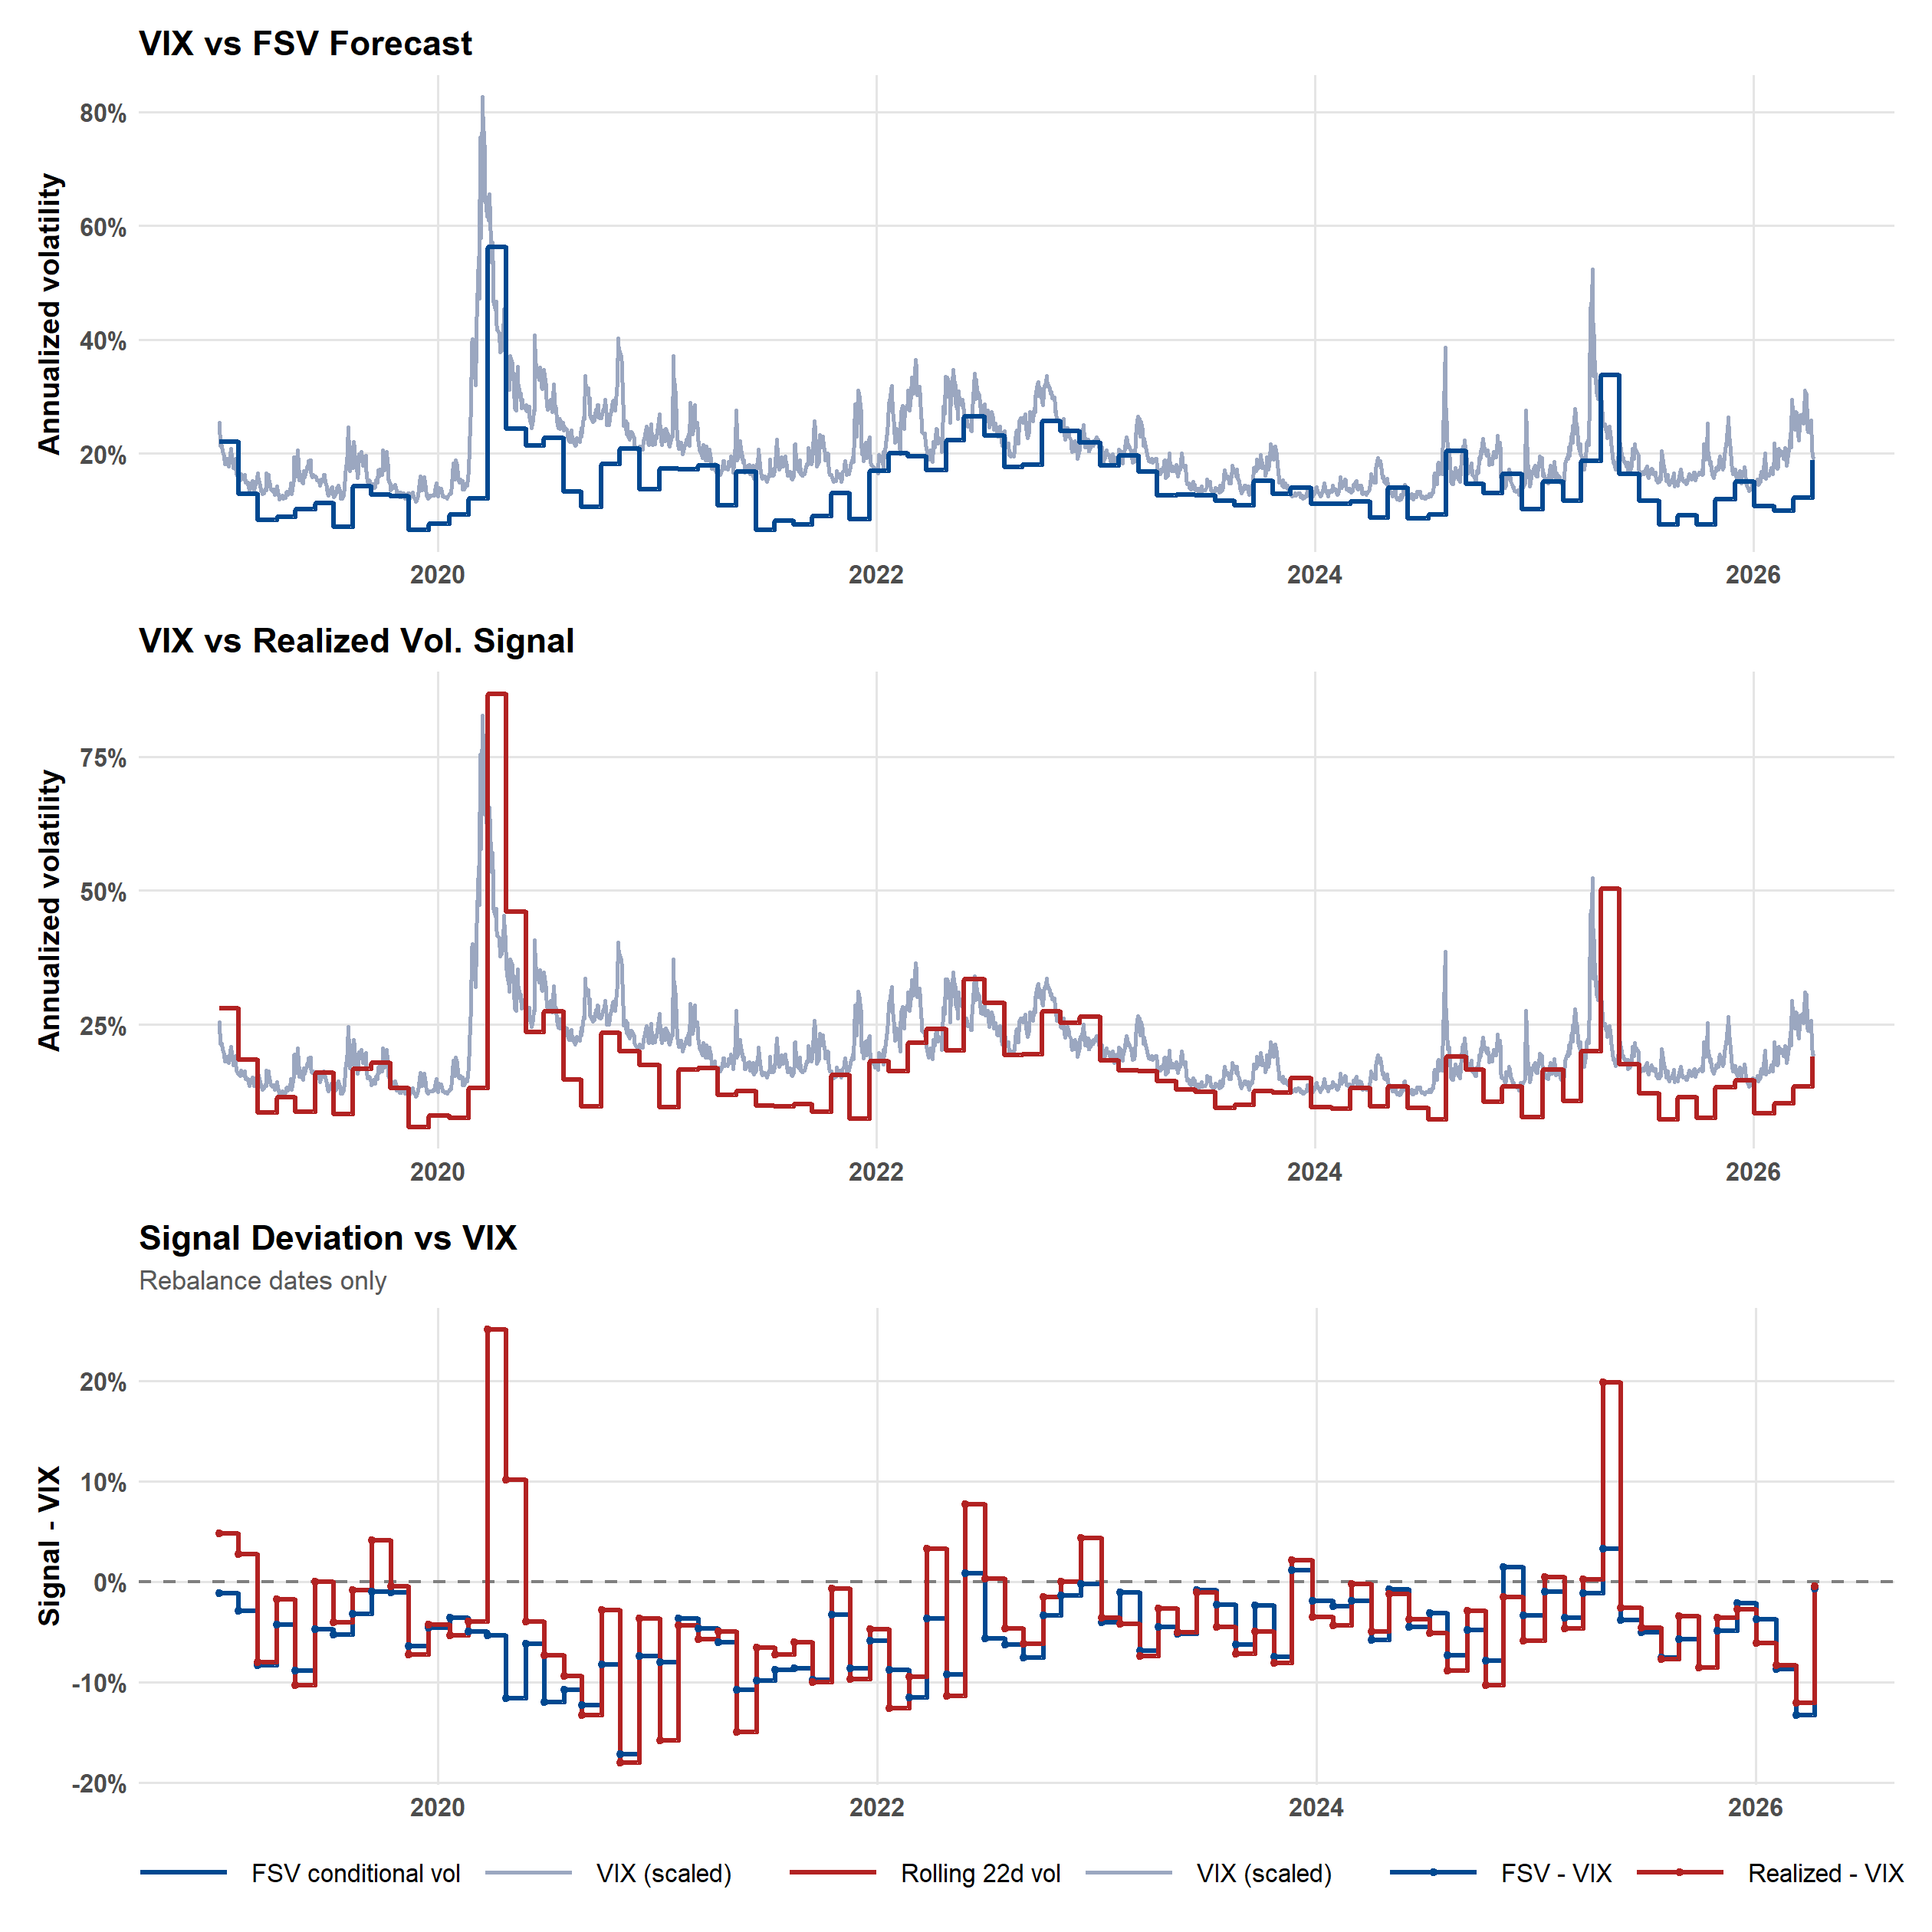
\includegraphics[width=0.54\textwidth]{../03_Results/Charts/part1_vix_signal_deviation_multiplot.png}
    \caption{Top: VIX vs.\ FSV forecast signal. Middle: VIX vs.\ realized-vol signal.
             Bottom: deviations (signal minus VIX), evaluated on rebalance dates.}
  \end{figure}

\end{frame}

%---- 5.3 - Part 1: Cumulative Return -----------------------------------------%

\begin{frame}{Part 1 -- SPY: Cumulative Return}

  \begin{figure}
    \centering
    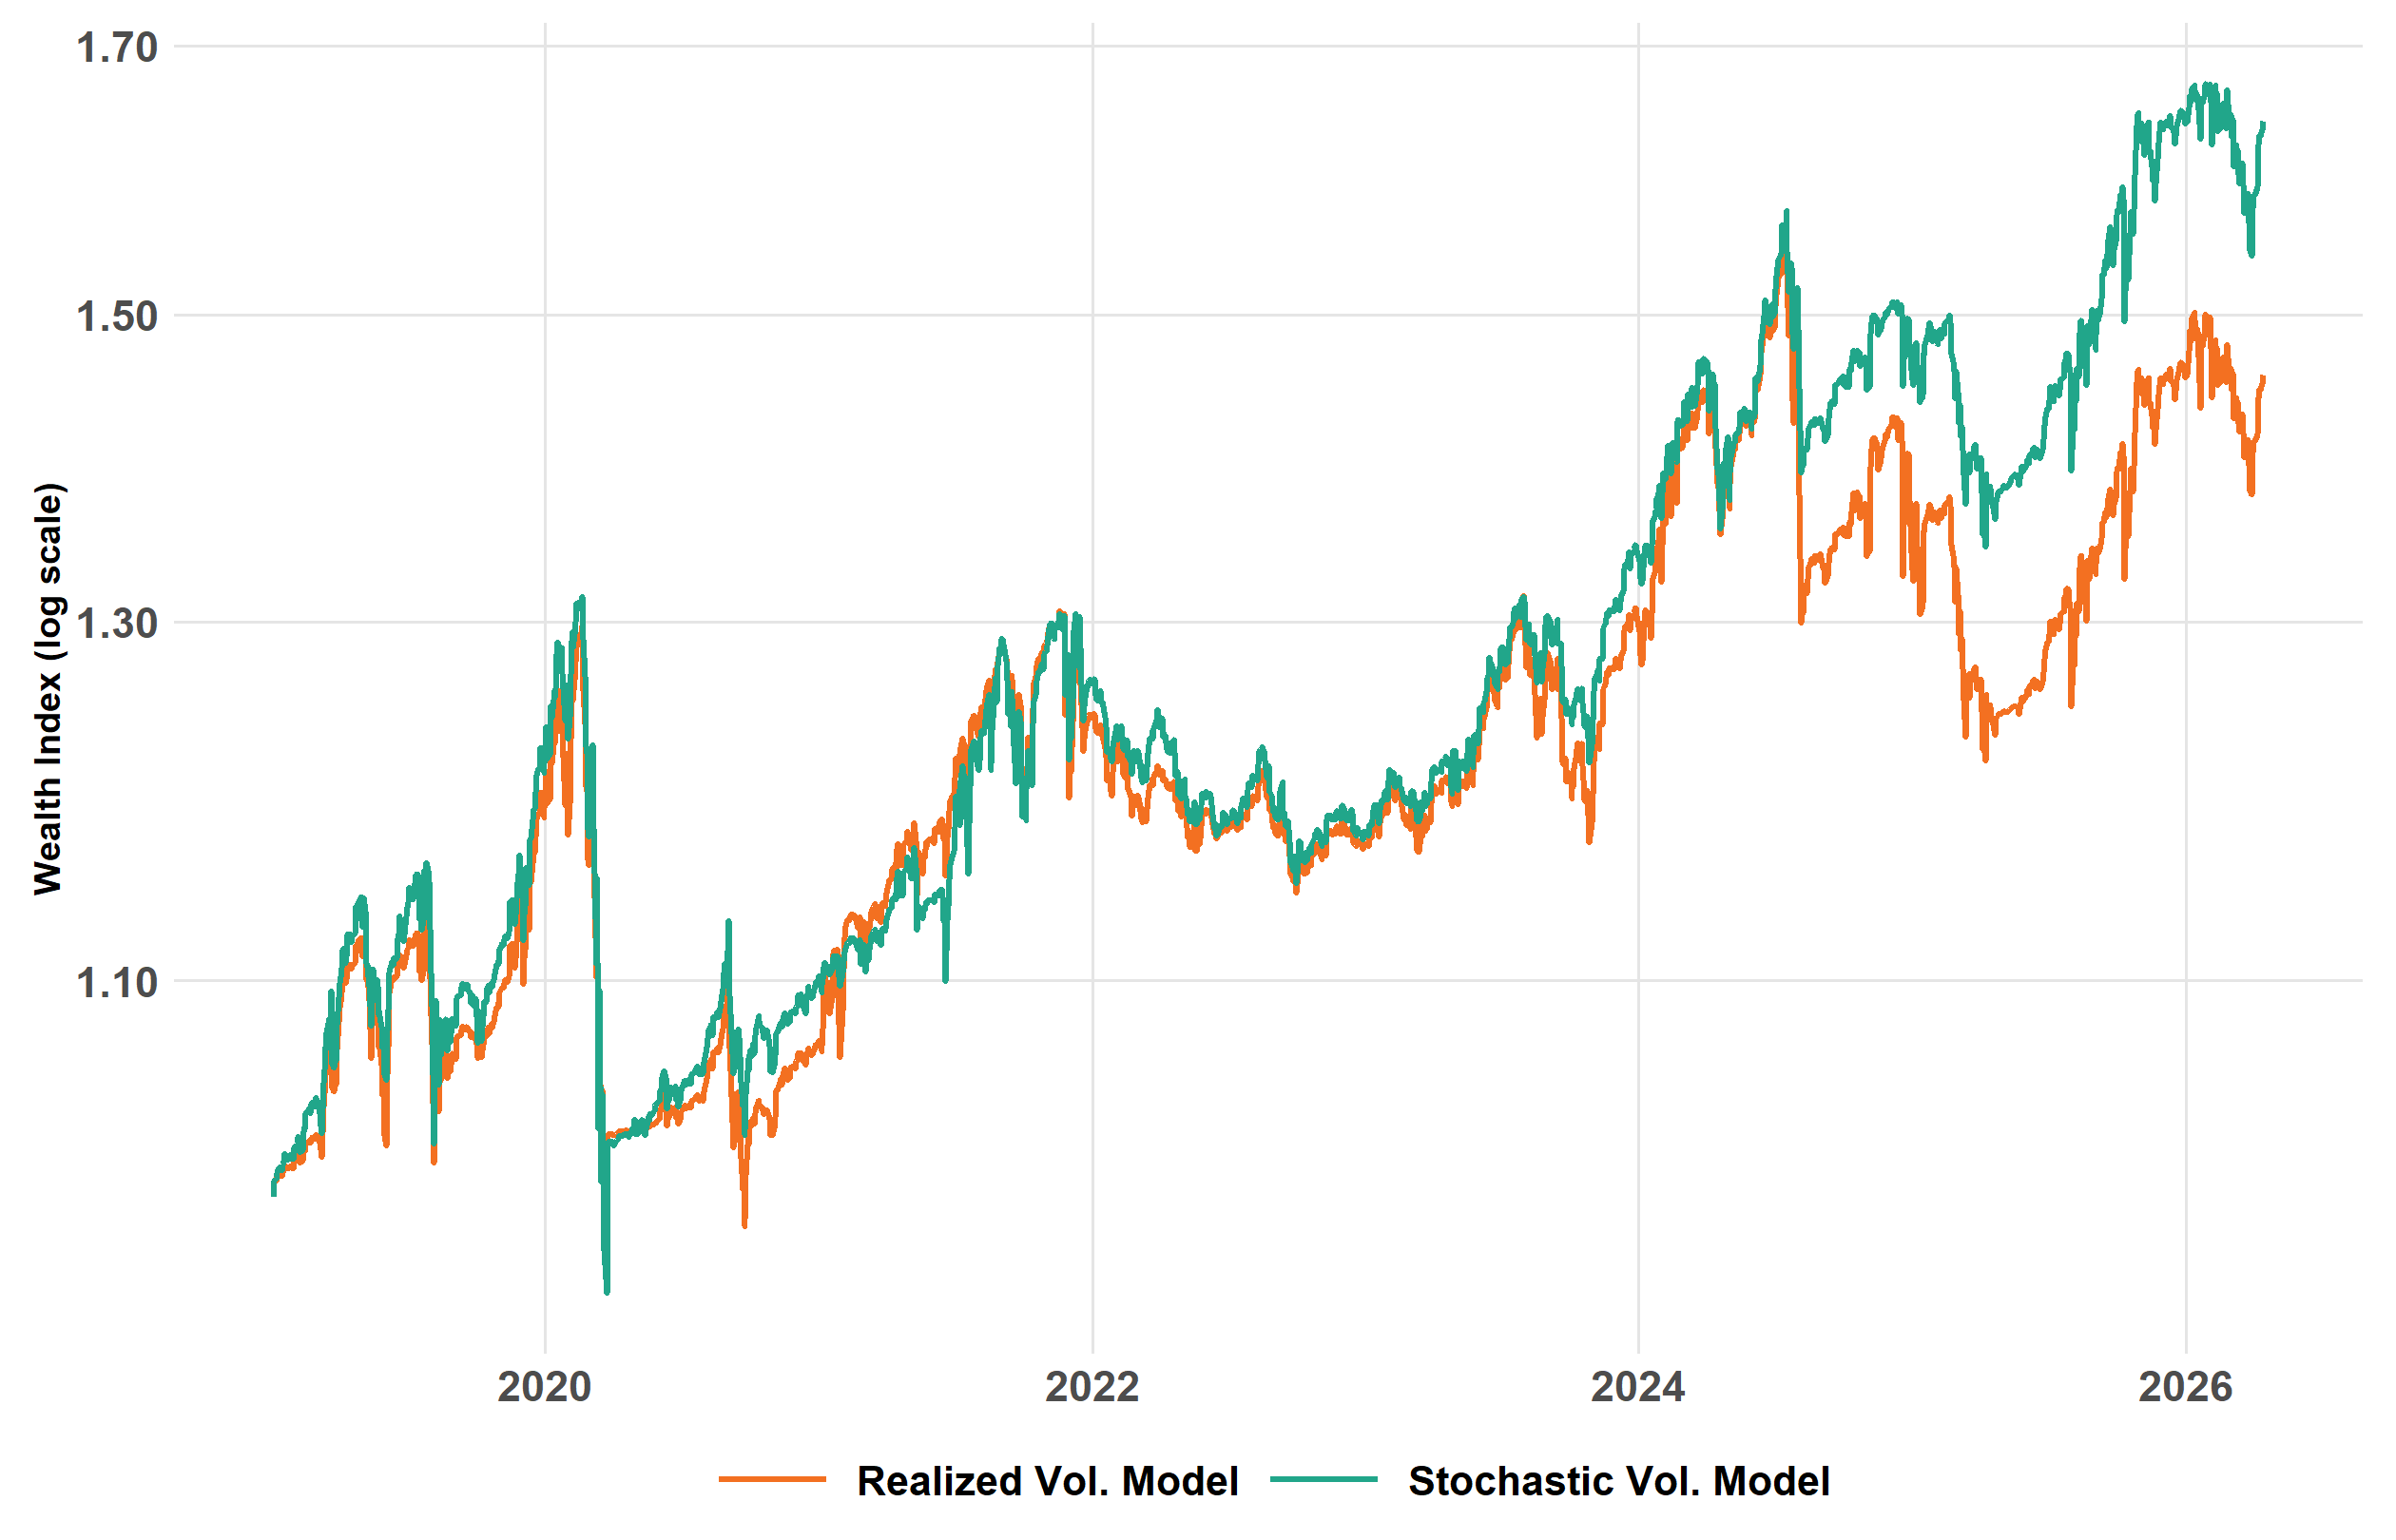
\includegraphics[width=0.92\textwidth]{../03_Results/Charts/part1_cumulative_return.png}
    \caption{Cumulative wealth index (log scale), Jan 2019 -- Dec 2024, 0 bps transaction costs,
             shown for managed models only.
             FSV Ret/Vol~0.496 vs.\ Realized Vol.\ Model~0.352; turnover 4.56 vs.\ 5.96.}
  \end{figure}

\end{frame}

%---- 5.35 - Part 1 Results (0 vs 5 bps) --------------------------------------%

\begin{frame}{Part 1 -- Results (0 vs 5 bps)}

  {\scriptsize \textbf{0 bps transaction cost}}

  \vspace{0.2em}
  {\scriptsize
  \setlength{\tabcolsep}{4pt}
  \begin{tabular}{@{}lrrrrr@{}}
    \toprule
    \textbf{Strategy} & \textbf{Return} & \textbf{Vol} & \textbf{Ret/Vol} & \textbf{MaxDD} & \textbf{Turnover} \\
    \midrule
    SPY Benchmark         & 16.8\% & 19.6\% & 0.859 & $-$33.7\% & 0.00 \\
    Realized Vol.\ Model  & 5.3\%  & 15.2\% & 0.352 & $-$25.8\% & 5.96 \\
    FSV                   & 7.1\%  & 14.3\% & 0.496 & $-$27.7\% & 4.56 \\
    \bottomrule
  \end{tabular}
  }

  \vspace{0.6em}
  {\scriptsize \textbf{5 bps transaction cost}}

  \vspace{0.2em}
  {\scriptsize
  \setlength{\tabcolsep}{4pt}
  \begin{tabular}{@{}lrrrrr@{}}
    \toprule
    \textbf{Strategy} & \textbf{Return} & \textbf{Vol} & \textbf{Ret/Vol} & \textbf{MaxDD} & \textbf{Turnover} \\
    \midrule
    SPY Benchmark         & 16.8\% & 19.6\% & 0.859 & $-$33.7\% & 0.00 \\
    Realized Vol.\ Model  & 5.0\%  & 15.2\% & 0.332 & $-$25.9\% & 5.96 \\
    FSV                   & 6.8\%  & 14.3\% & 0.479 & $-$27.7\% & 4.56 \\
    \bottomrule
  \end{tabular}
  }

\end{frame}

%---- 5.4 - Part 2 methodology moved here per requested order -----------------%

\begin{frame}{Part 2 Methodology: Exact Weight Construction}

  \textbf{Covariance forecast at rebalance time $t$:}
  \begin{itemize}
    \item Realized-vol model: rolling 22-day sample covariance, $\hat{\Sigma}^{\text{roll}}_t$
    \item Stochastic-vol model: FSV one-step-ahead covariance, $\hat{\Sigma}^{\text{fsv}}_{t+1|t}$
  \end{itemize}

  \textbf{Expected return estimate (causal):}
  \[
    \hat{\mu}_t = \frac{1}{t}\sum_{s=1}^{t} r_s
  \]

  \textbf{Within each bucket (equity, bonds, gold), solve long-only mean-variance:}
  \[
    \max_{w}\; w^\top \hat{\mu}_t - \frac{\lambda}{2}w^\top \hat{\Sigma}_t w
  \]
  subject to
  \[
    w_i \ge 0,\qquad \sum_i w_i = 1, \qquad \lambda = 10
  \]
  implemented via $w=\mathrm{softmax}(z)$ with optimizer bounds $z_j \in [-20,20]$.

  \vspace{0.4em}
  Bucket solutions are scaled by fixed top-level budgets:
  \[
    \text{pf1}: (0.45,0.45,0.10),\qquad \text{pf2}: (0.60,0.40,0.00)
  \]

\end{frame}

\begin{frame}{Boundaries and Return Construction}

  \textbf{Weight boundaries}
  \begin{itemize}
    \item Part 1: scalar SPY weight constrained to $w_t \in [0,2]$.
    \item Part 2: long-only simplex constraints ($w_i \ge 0$, weights sum to 1 in each bucket and overall), implemented numerically with $z_j \in [-20,20]$.
  \end{itemize}

  \textbf{Gross returns}
  \[
    r^{\text{gross}}_{t+1,\text{Part1}} = w_t \, r_{\text{SPY},t+1}, \qquad
    r^{\text{gross}}_{t+1,\text{Part2}} = w_t^\top r_{t+1}
  \]

  \textbf{Financing cost for leverage}
  \[
    \text{FC}_{t+1} =
    \max(0,\text{gross exposure}_t-1)\left(r_{\text{SHY},t+1}+\frac{0.003}{252}\right)
  \]
  with floor at zero implied by the borrowing-rate proxy.

  \textbf{Net returns with transaction costs}
  \[
    r^{\text{net}}_{t+1} =
    r^{\text{gross}}_{t+1} - \text{FC}_{t+1} - \frac{\text{tcost}_{\text{bps}}}{10{,}000}\cdot \text{turnover}_t
  \]
  where transaction costs are evaluated at 0 and 5 bps, and one-way turnover is
  \[
    \text{turnover}_t =
    \begin{cases}
      |w_t-w_{t-1}|, & \text{Part 1 (single weight)}\\
      \frac{1}{2}\sum_i |w_{i,t}-w_{i,t-1}|, & \text{Part 2 (portfolio weights)}
    \end{cases}
  \]
  measured only on rebalance dates (weights are held constant between rebalances).

\end{frame}

%---- 5.5 - Part 2: Multi-Asset Cumulative Return -----------------------------%

\begin{frame}{Part 2 -- Multi-Asset: Cumulative Return}

  \begin{figure}
    \centering
    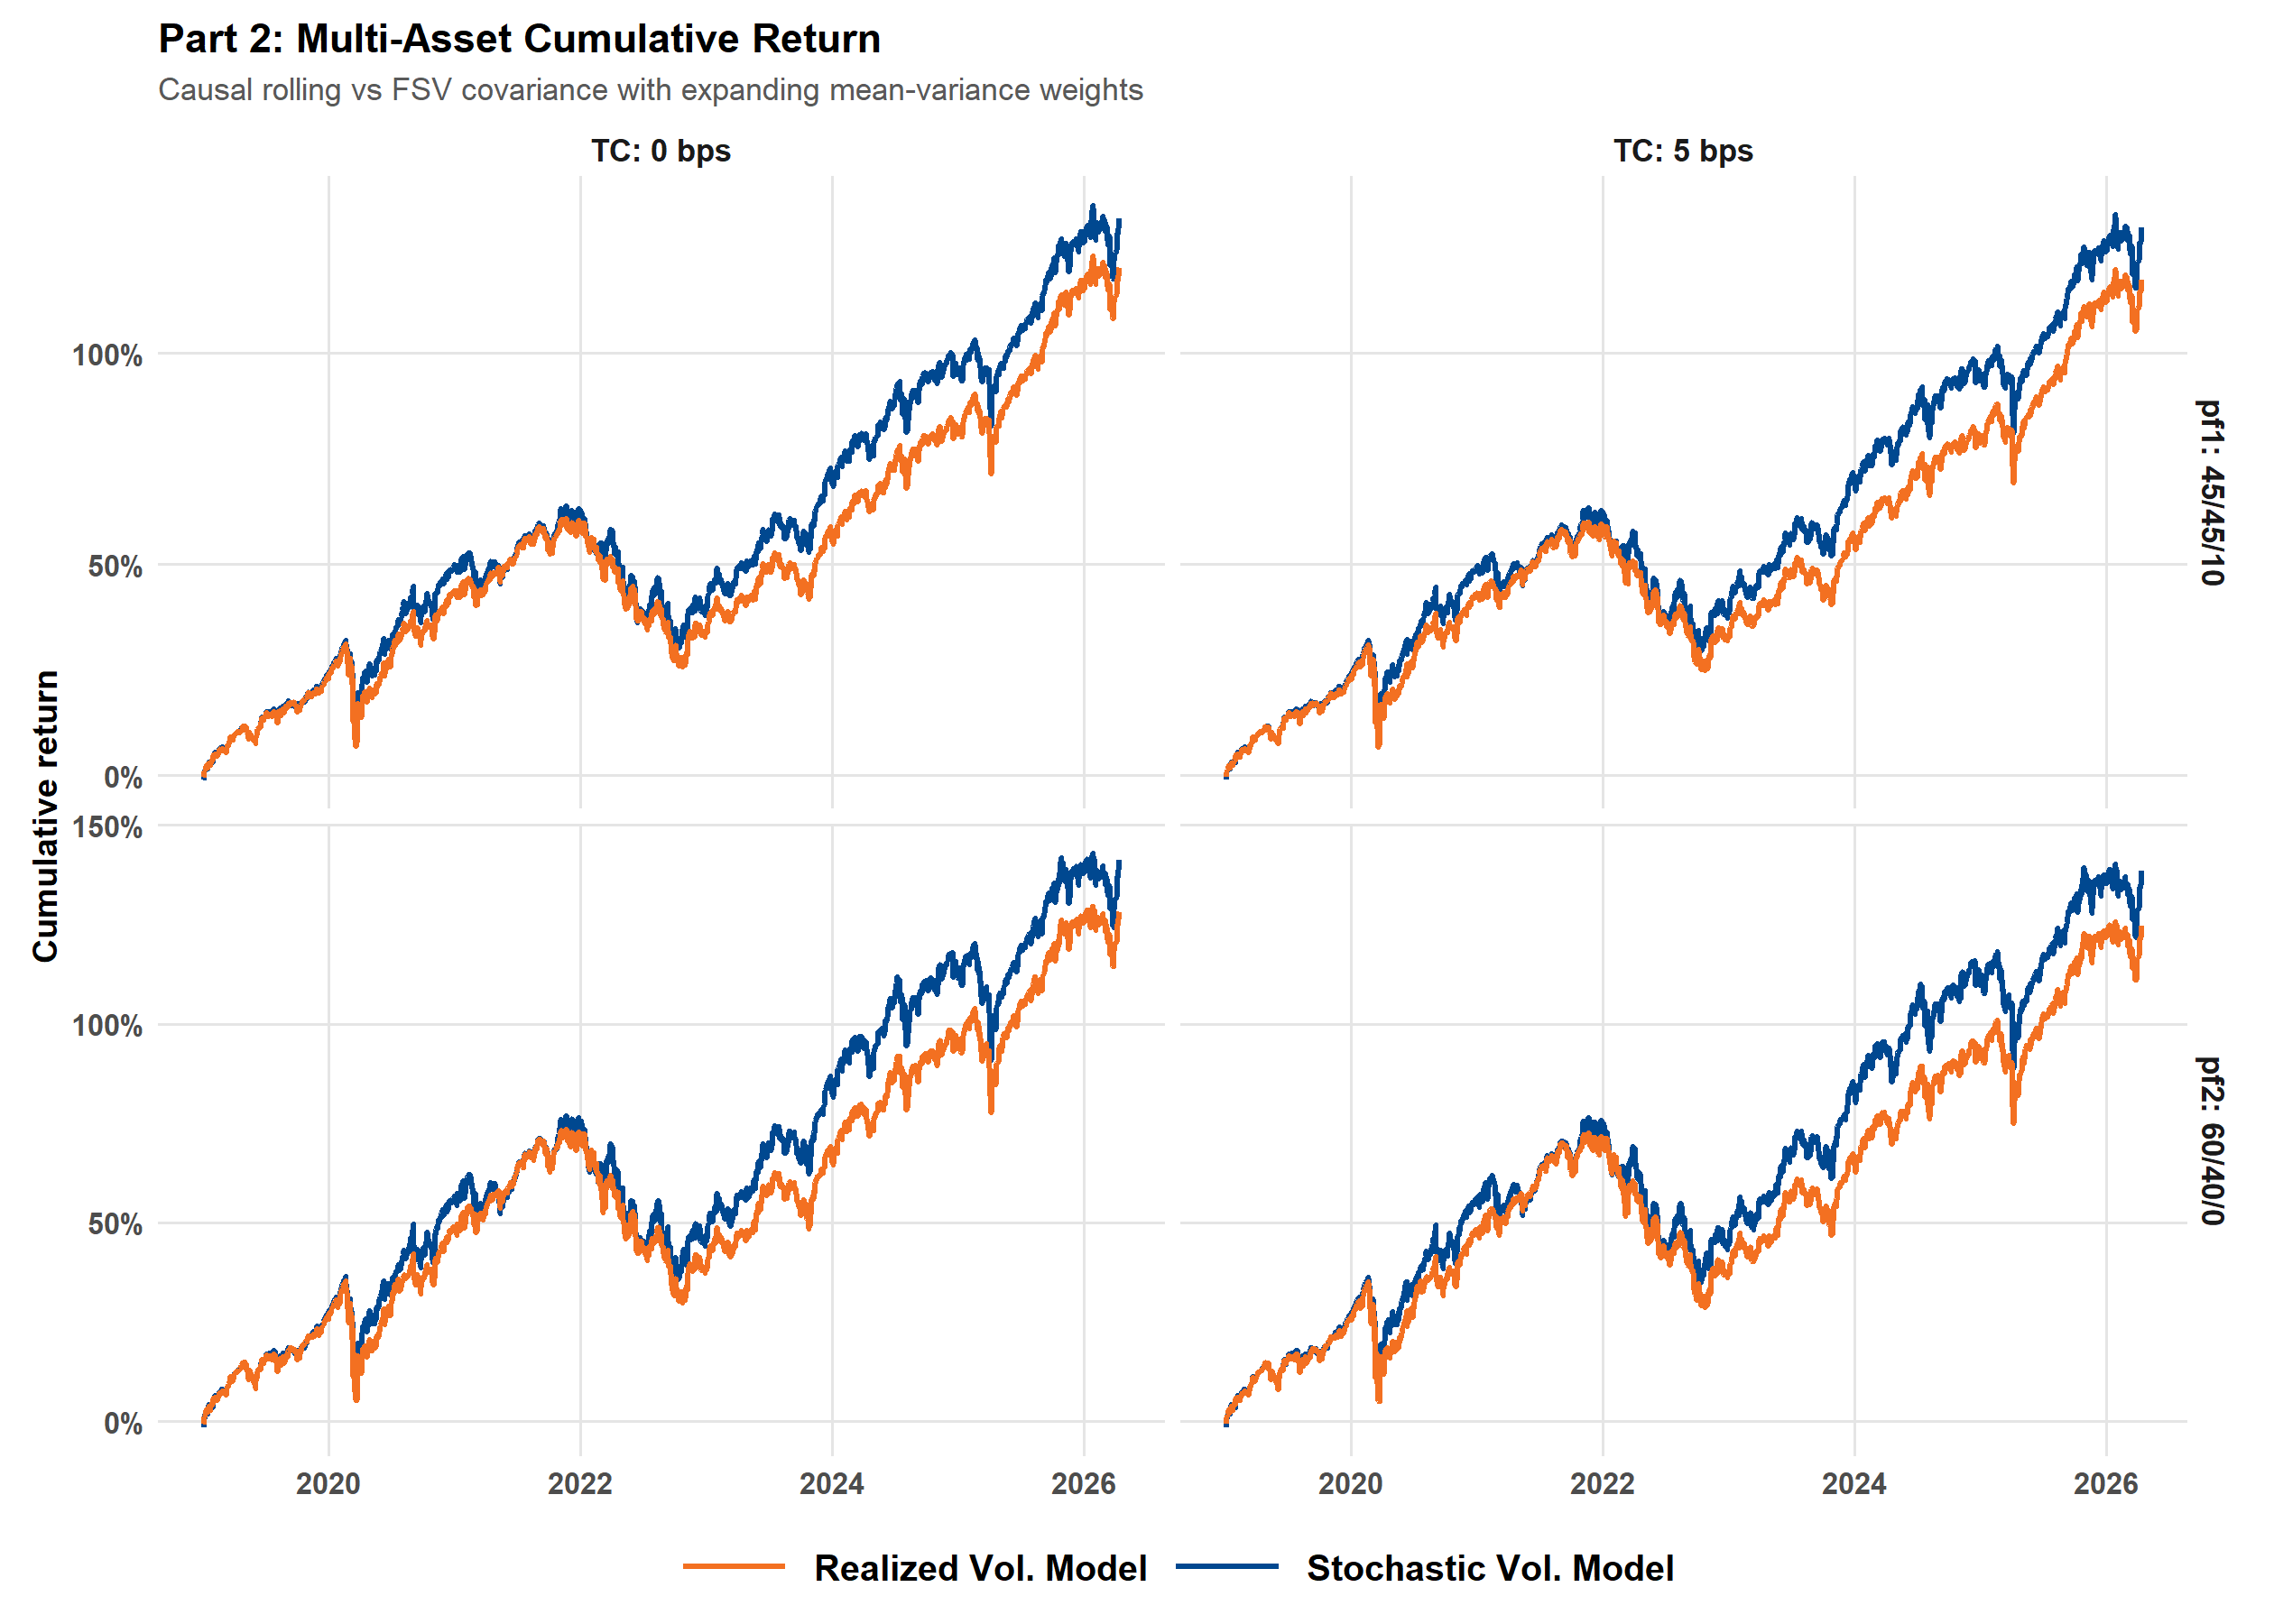
\includegraphics[width=0.92\textwidth]{../03_Results/Charts/part2_cumulative_return.png}
    \caption{Cumulative return for budget portfolios pf1 (45/45/10) and pf2 (60/40/0),
             0 bps transaction costs.
             Legend labels: Stochastic Vol.\ Model and Realized Vol.\ Model.}
  \end{figure}

\end{frame}

%---- 5.5 - Part 2: Equity Weight Over Time -----------------------------------%

\begin{frame}{Part 2 -- Multi-Asset: Portfolio Weight Dynamics}

  \begin{figure}
    \centering
    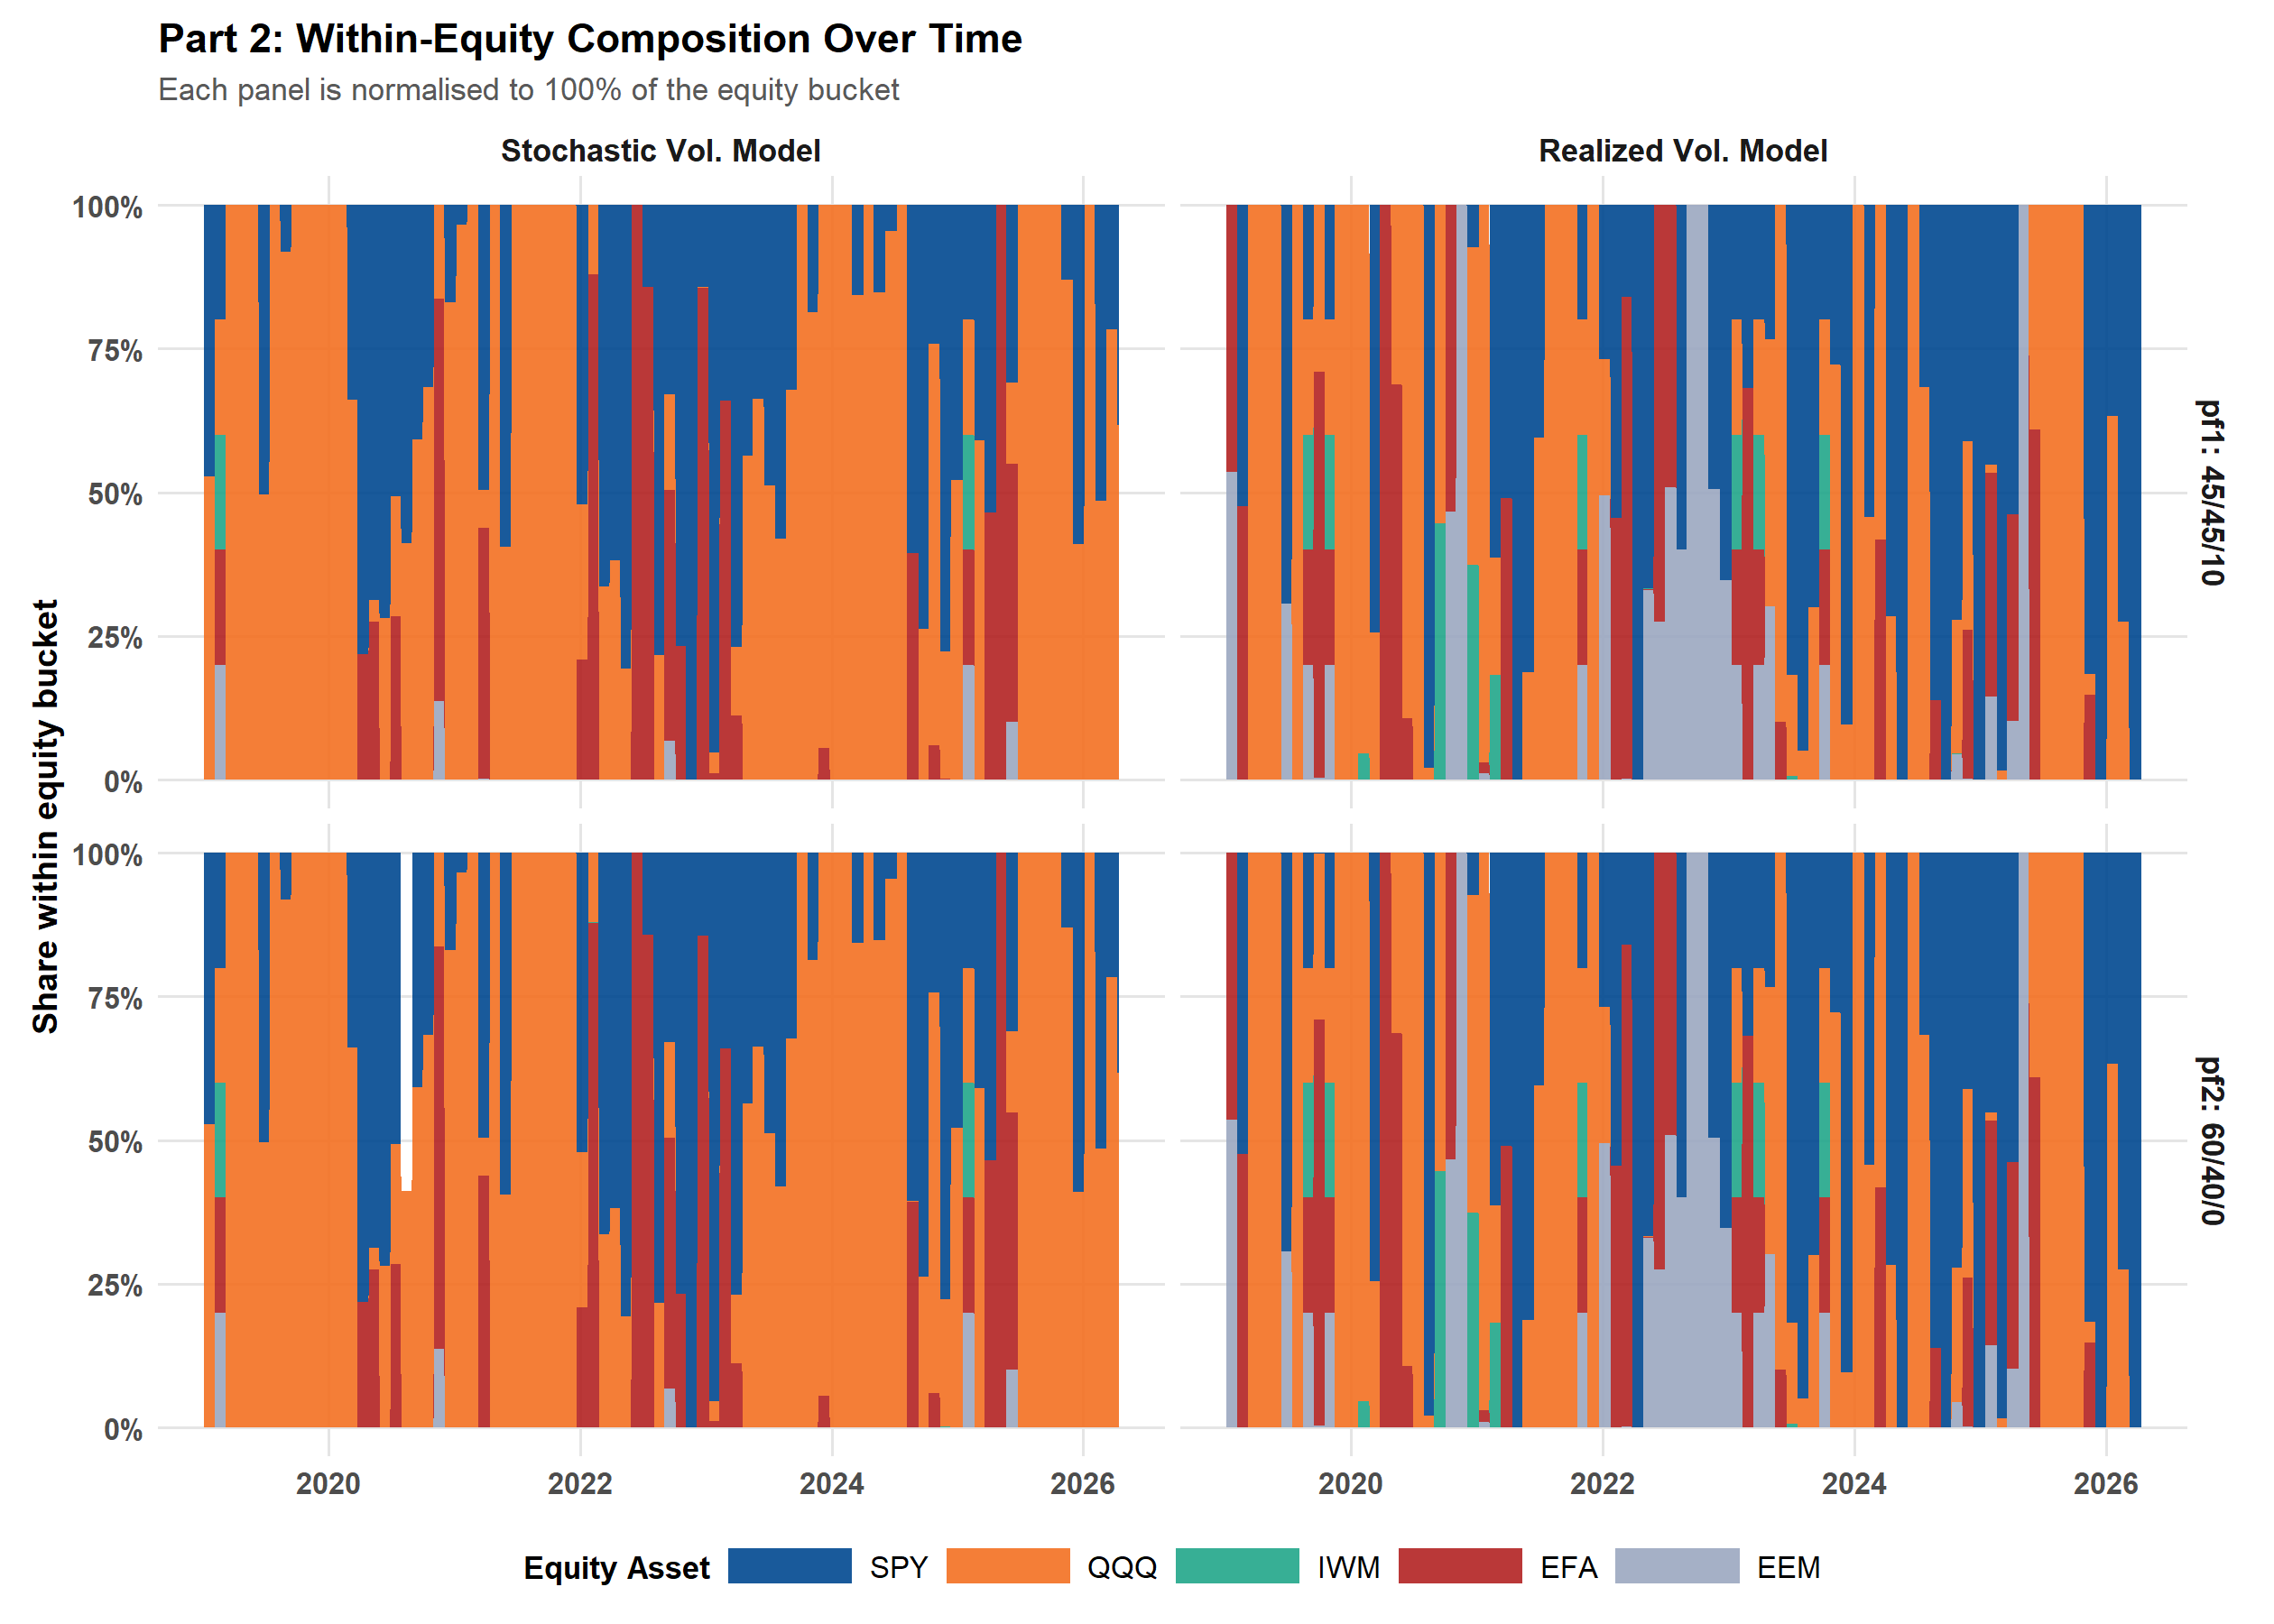
\includegraphics[width=0.92\textwidth]{../03_Results/Charts/part2_equity_within_bucket_composition.png}
    \caption{Within-equity composition over time (normalised to 100\% within the equity bucket),
             by budget (pf1/pf2) and model (Realized Vol.\ Model vs Stochastic Vol.\ Model).}
  \end{figure}

\end{frame}

%---- 5.6 - Part 1 Results (0 vs 5 bps) ---------------------------------------%

%---- 5.7 - Part 2 Results (0 vs 5 bps) ---------------------------------------%

\begin{frame}{Part 2 -- Results (0 vs 5 bps)}

  {\scriptsize \textbf{0 bps transaction cost}}

  \vspace{0.2em}
  {\scriptsize
  \setlength{\tabcolsep}{4pt}
  \begin{tabular}{@{}llrrrrr@{}}
    \toprule
    \textbf{Budget} & \textbf{Strategy} & \textbf{Return} & \textbf{Vol} & \textbf{Ret/Vol} & \textbf{MaxDD} & \textbf{Turnover} \\
    \midrule
    pf1 & Realized Vol.\ Model   & 11.5\% & 10.5\% & 1.097 & $-$21.9\% & 3.78 \\
    pf1 & Stochastic Vol.\ Model & 12.3\% & 11.3\% & 1.089 & $-$20.9\% & 2.73 \\
    pf2 & Realized Vol.\ Model   & 12.0\% & 12.8\% & 0.942 & $-$25.3\% & 4.54 \\
    pf2 & Stochastic Vol.\ Model & 12.9\% & 13.7\% & 0.939 & $-$23.5\% & 3.24 \\
    \bottomrule
  \end{tabular}
  }

  \vspace{0.55em}
  {\scriptsize \textbf{5 bps transaction cost}}

  \vspace{0.2em}
  {\scriptsize
  \setlength{\tabcolsep}{4pt}
  \begin{tabular}{@{}llrrrrr@{}}
    \toprule
    \textbf{Budget} & \textbf{Strategy} & \textbf{Return} & \textbf{Vol} & \textbf{Ret/Vol} & \textbf{MaxDD} & \textbf{Turnover} \\
    \midrule
    pf1 & Realized Vol.\ Model   & 11.3\% & 10.5\% & 1.077 & $-$22.0\% & 3.78 \\
    pf1 & Stochastic Vol.\ Model & 12.1\% & 11.3\% & 1.075 & $-$21.0\% & 2.73 \\
    pf2 & Realized Vol.\ Model   & 11.8\% & 12.8\% & 0.922 & $-$25.5\% & 4.54 \\
    pf2 & Stochastic Vol.\ Model & 12.7\% & 13.7\% & 0.925 & $-$23.7\% & 3.24 \\
    \bottomrule
  \end{tabular}
  }

\end{frame}

%---- 5.8 - Discussion & Caveats ----------------------------------------------%

\begin{frame}{Discussion \& Caveats}

  \begin{block}{Main Findings}
    \begin{itemize}
      \setlength\itemsep{0.4em}
      \item \textbf{RQ 1 (Single Asset):} FSV scaling \textit{improves upon} na\"{i}ve M\&M ---
            better risk-adjusted returns, lower drawdown, and lower turnover. However,
            neither beats buy-and-hold in the 2019--2024 low-VIX regime, consistent
            with M\&M's own observation that alpha is regime-dependent.
      \item \textbf{RQ 2 (Multi-Asset):} FSV covariance forecasts yield a
            \textit{practically superior} portfolio on return, drawdown, and turnover
            at both budgets, with the largest advantage being \textbf{transaction-cost efficiency}.
    \end{itemize}
  \end{block}

  \begin{alertblock}{Key Caveats \& Deviations}
    \begin{itemize}
      \setlength\itemsep{0.3em}
      \item \textbf{Test window:} Jan 2019 onward; GFC and pre-2019 crises are
            \textit{not} in the evaluation period.
      \item \textbf{Leverage:} Scaling constant $c$ is calibrated on the full
            training window; realised exposures are dynamic and occasionally hit the 2$\times$ cap
            (mean exposure: Realized Vol.\ Model~$0.80\times$, FSV~$0.78\times$).
      \item \textbf{AR(1) SV estimation:} Parameters estimated by OLS on
            posterior-mean log-variance paths for tractability.
      \item \textbf{Funding cost:} Borrowing modelled as SHY daily return
            $+$ 30 bps spread, floored at zero.
      \item \textbf{Expected returns:} Expanding historical mean --- no alpha signal.
    \end{itemize}
  \end{alertblock}

\end{frame}

%---- moved from appendix: requested after slide 19 ---------------------------%

\begin{frame}{Appendix -- FSV Volatility: Local vs GCP}

  \begin{figure}
    \centering
    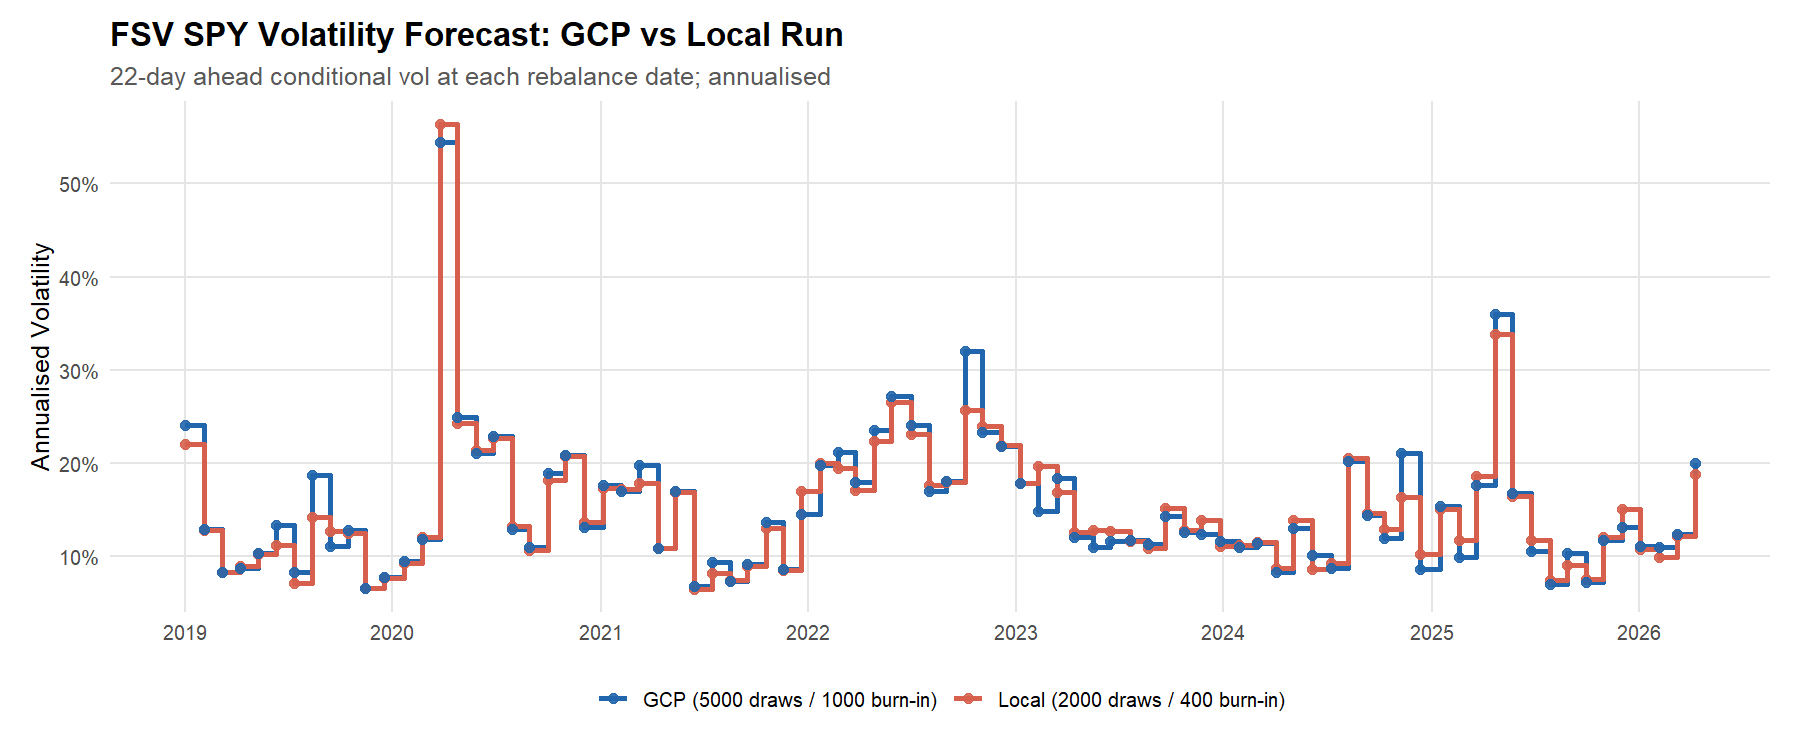
\includegraphics[width=0.92\textwidth]{../05_Results_NewRun/fsv_vol_gcp_vs_local.png}
    \caption{Comparison of Part 1 FSV volatility signal under local vs GCP MCMC settings.}
  \end{figure}

\end{frame}

%==== APPENDIX ================================================================%

\appendix

\section*{Appendix}

%---- A.1 - Rolling Return/Vol Ratio: Part 1 ----------------------------------%

\begin{frame}{Appendix -- Part 1: Rolling 252-Day Return/Volatility Ratio}

  \begin{figure}
    \centering
    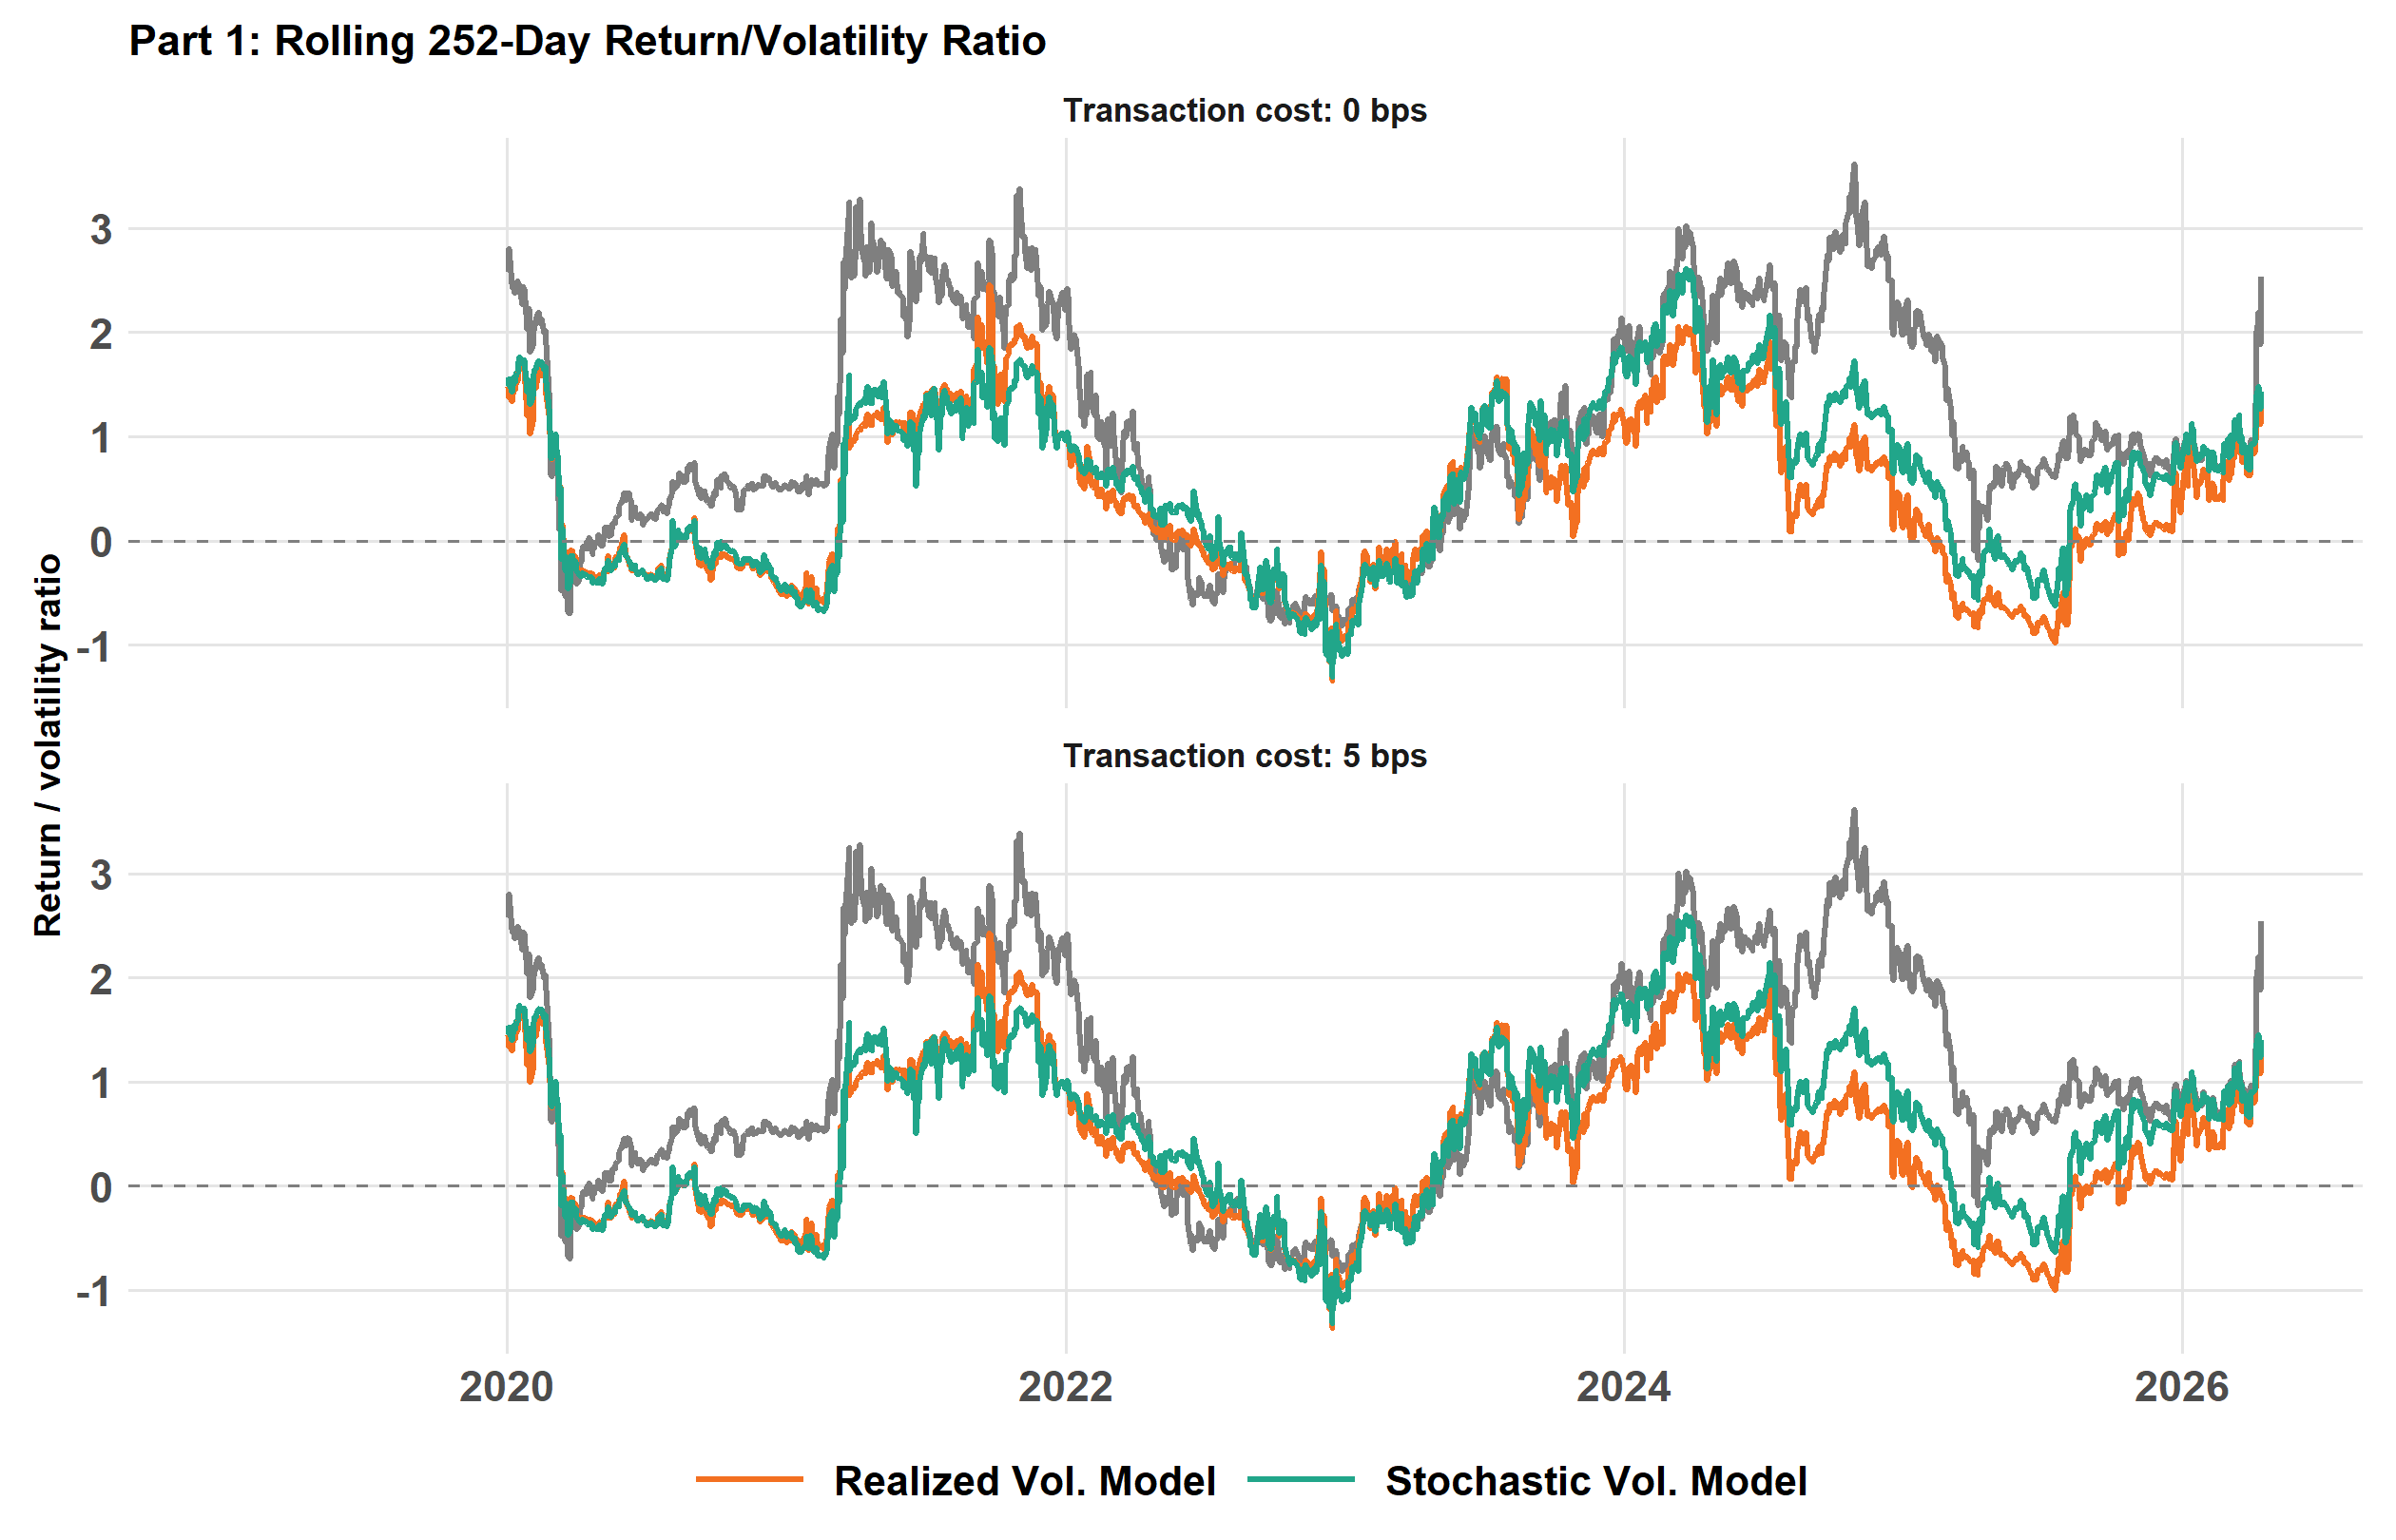
\includegraphics[width=0.92\textwidth]{../03_Results/Charts/part1_rolling_252_ratio.png}
    \caption{Rolling 252-day annualised return/volatility ratio for SPY strategies
             (top panel: 0 bps; bottom panel: 5 bps transaction costs).
             FSV consistently outperforms na\"{i}ve M\&M through the sample.}
  \end{figure}

\end{frame}

%---- A.2 - Rolling Return/Vol Ratio: Part 2 ----------------------------------%

\begin{frame}{Appendix -- Part 2: Rolling 252-Day Return/Volatility Ratio}

  \begin{figure}
    \centering
    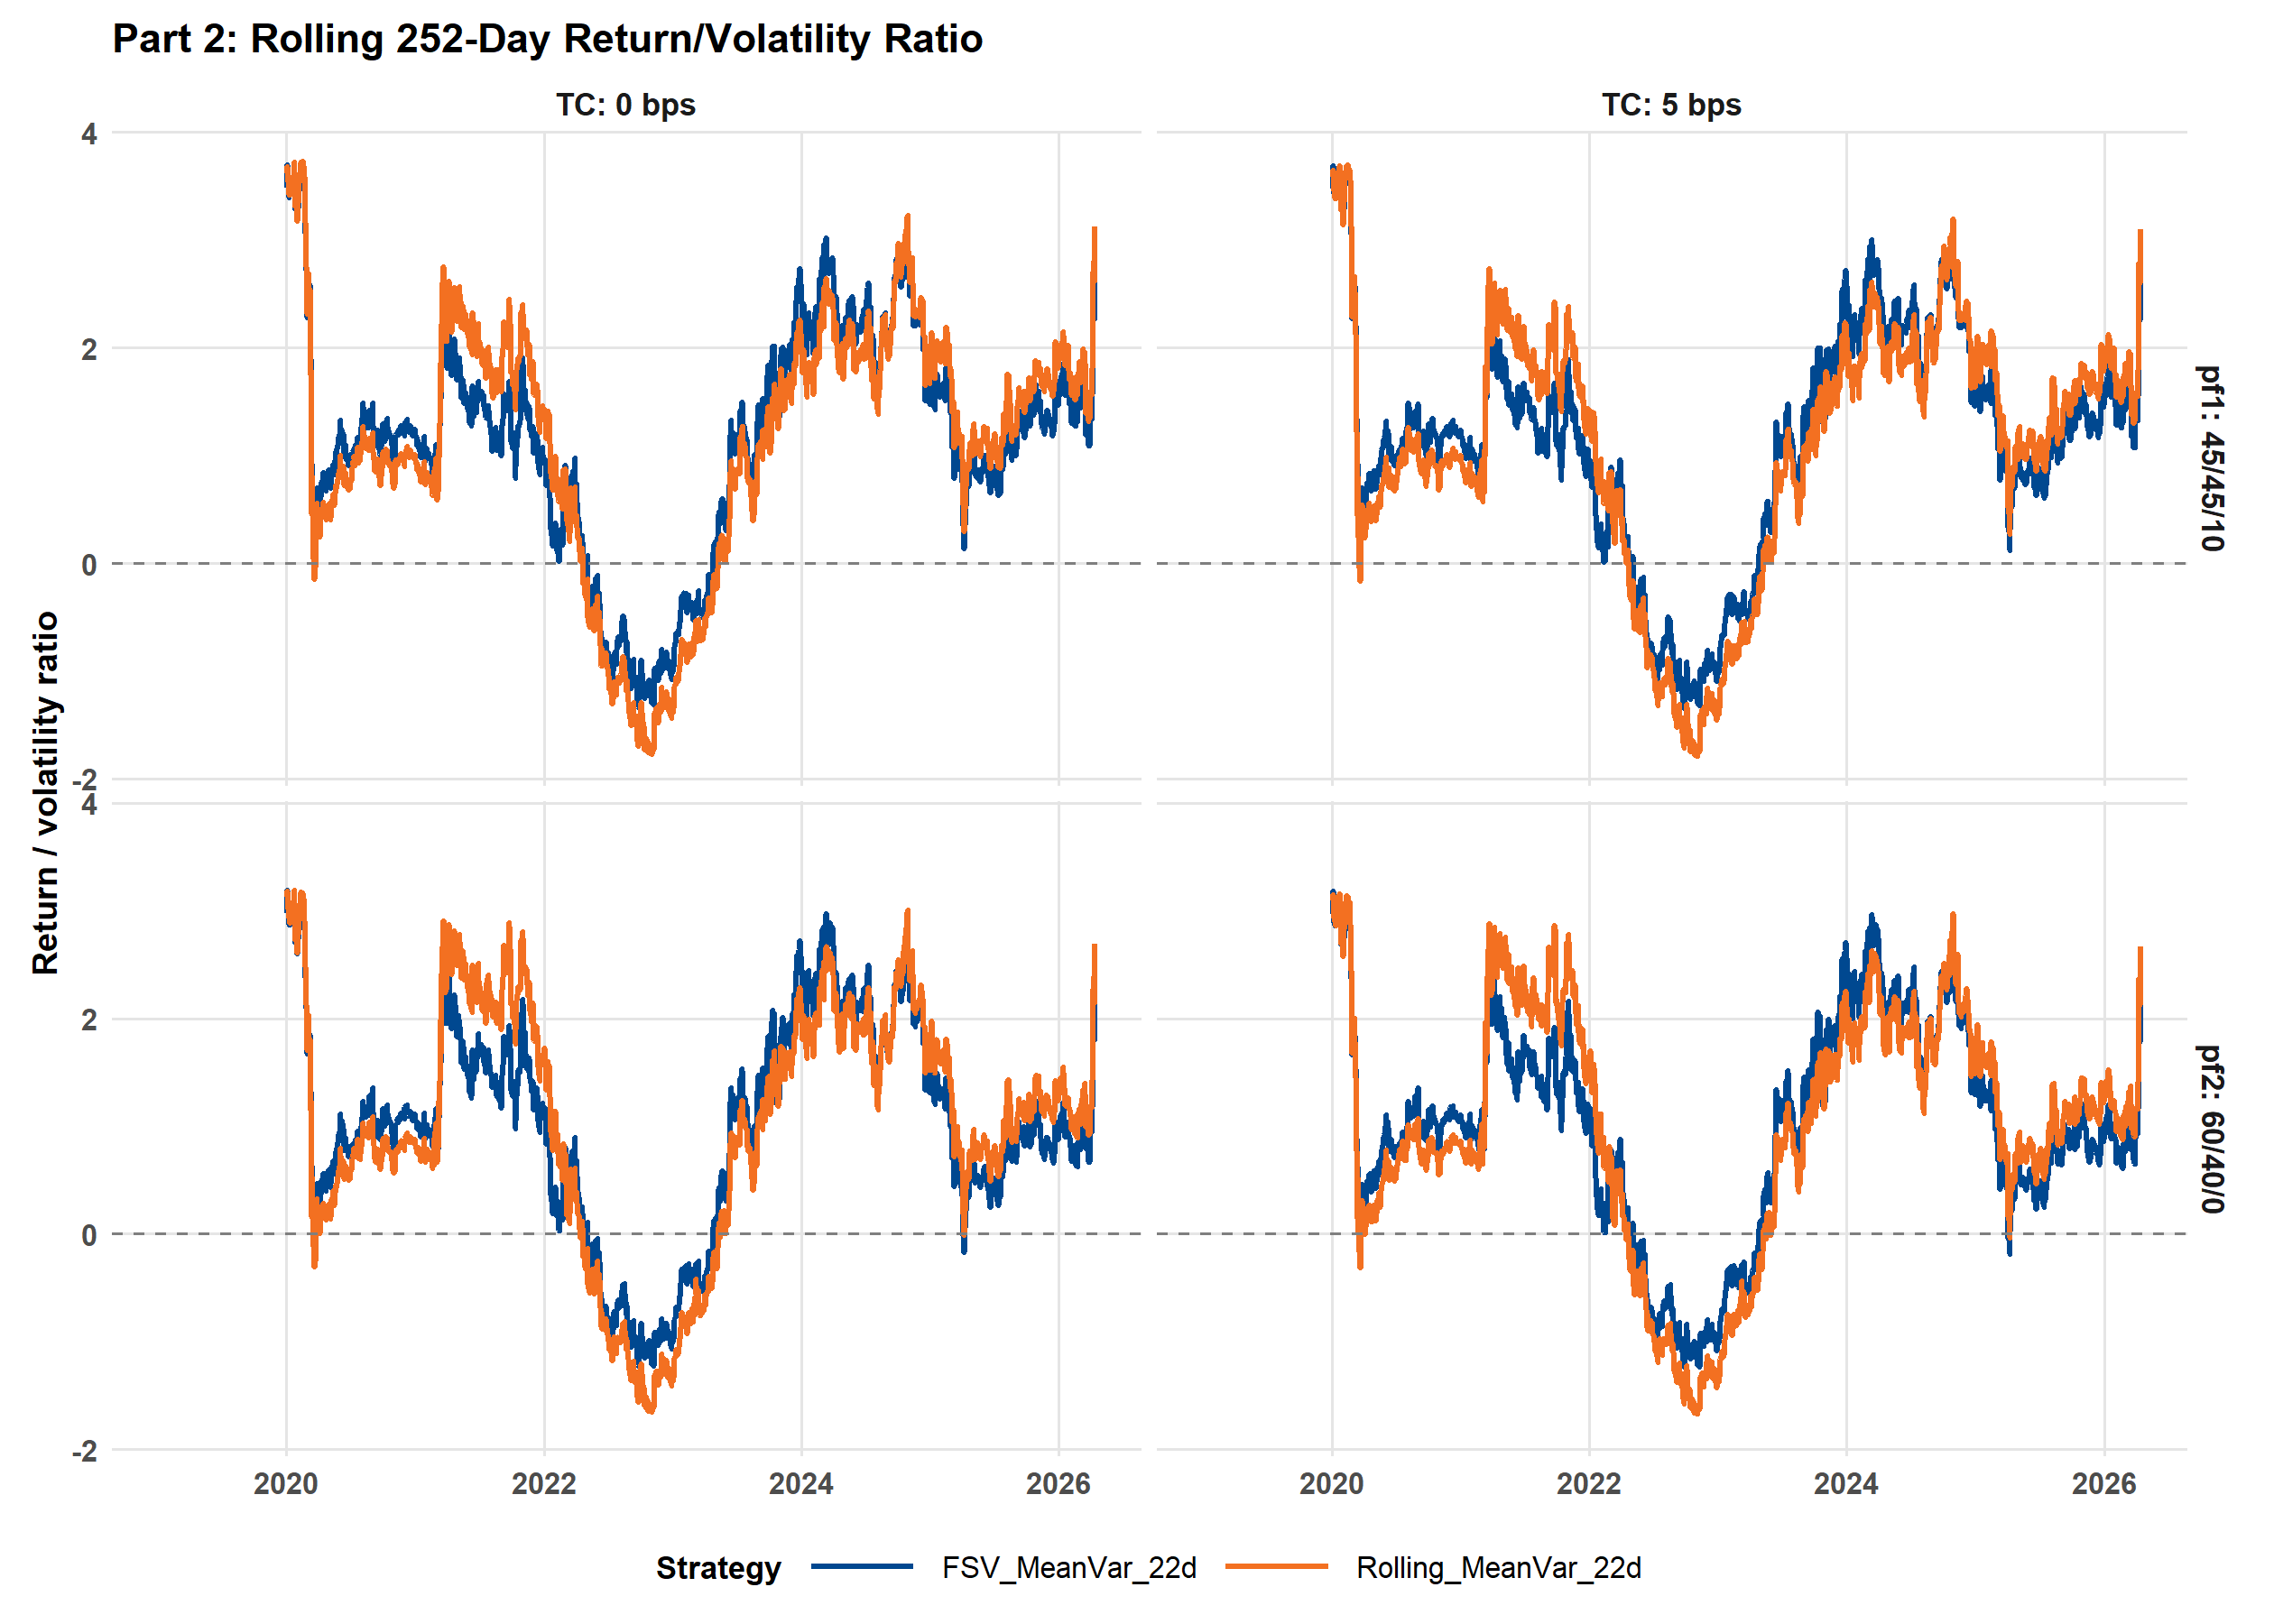
\includegraphics[width=0.92\textwidth]{../03_Results/Charts/part2_rolling_252_ratio.png}
    \caption{Rolling 252-day annualised return/volatility ratio for the multi-asset
             budget portfolios.
             Rows: pf1 (45/45/10) and pf2 (60/40/0); columns: 0 and 5 bps costs.}
  \end{figure}

\end{frame}

%---- A.3 - Global Minimum-Variance: Cumulative Return ------------------------%

\begin{frame}{Appendix -- Global Minimum-Variance: Cumulative Return}

  \begin{figure}
    \centering
    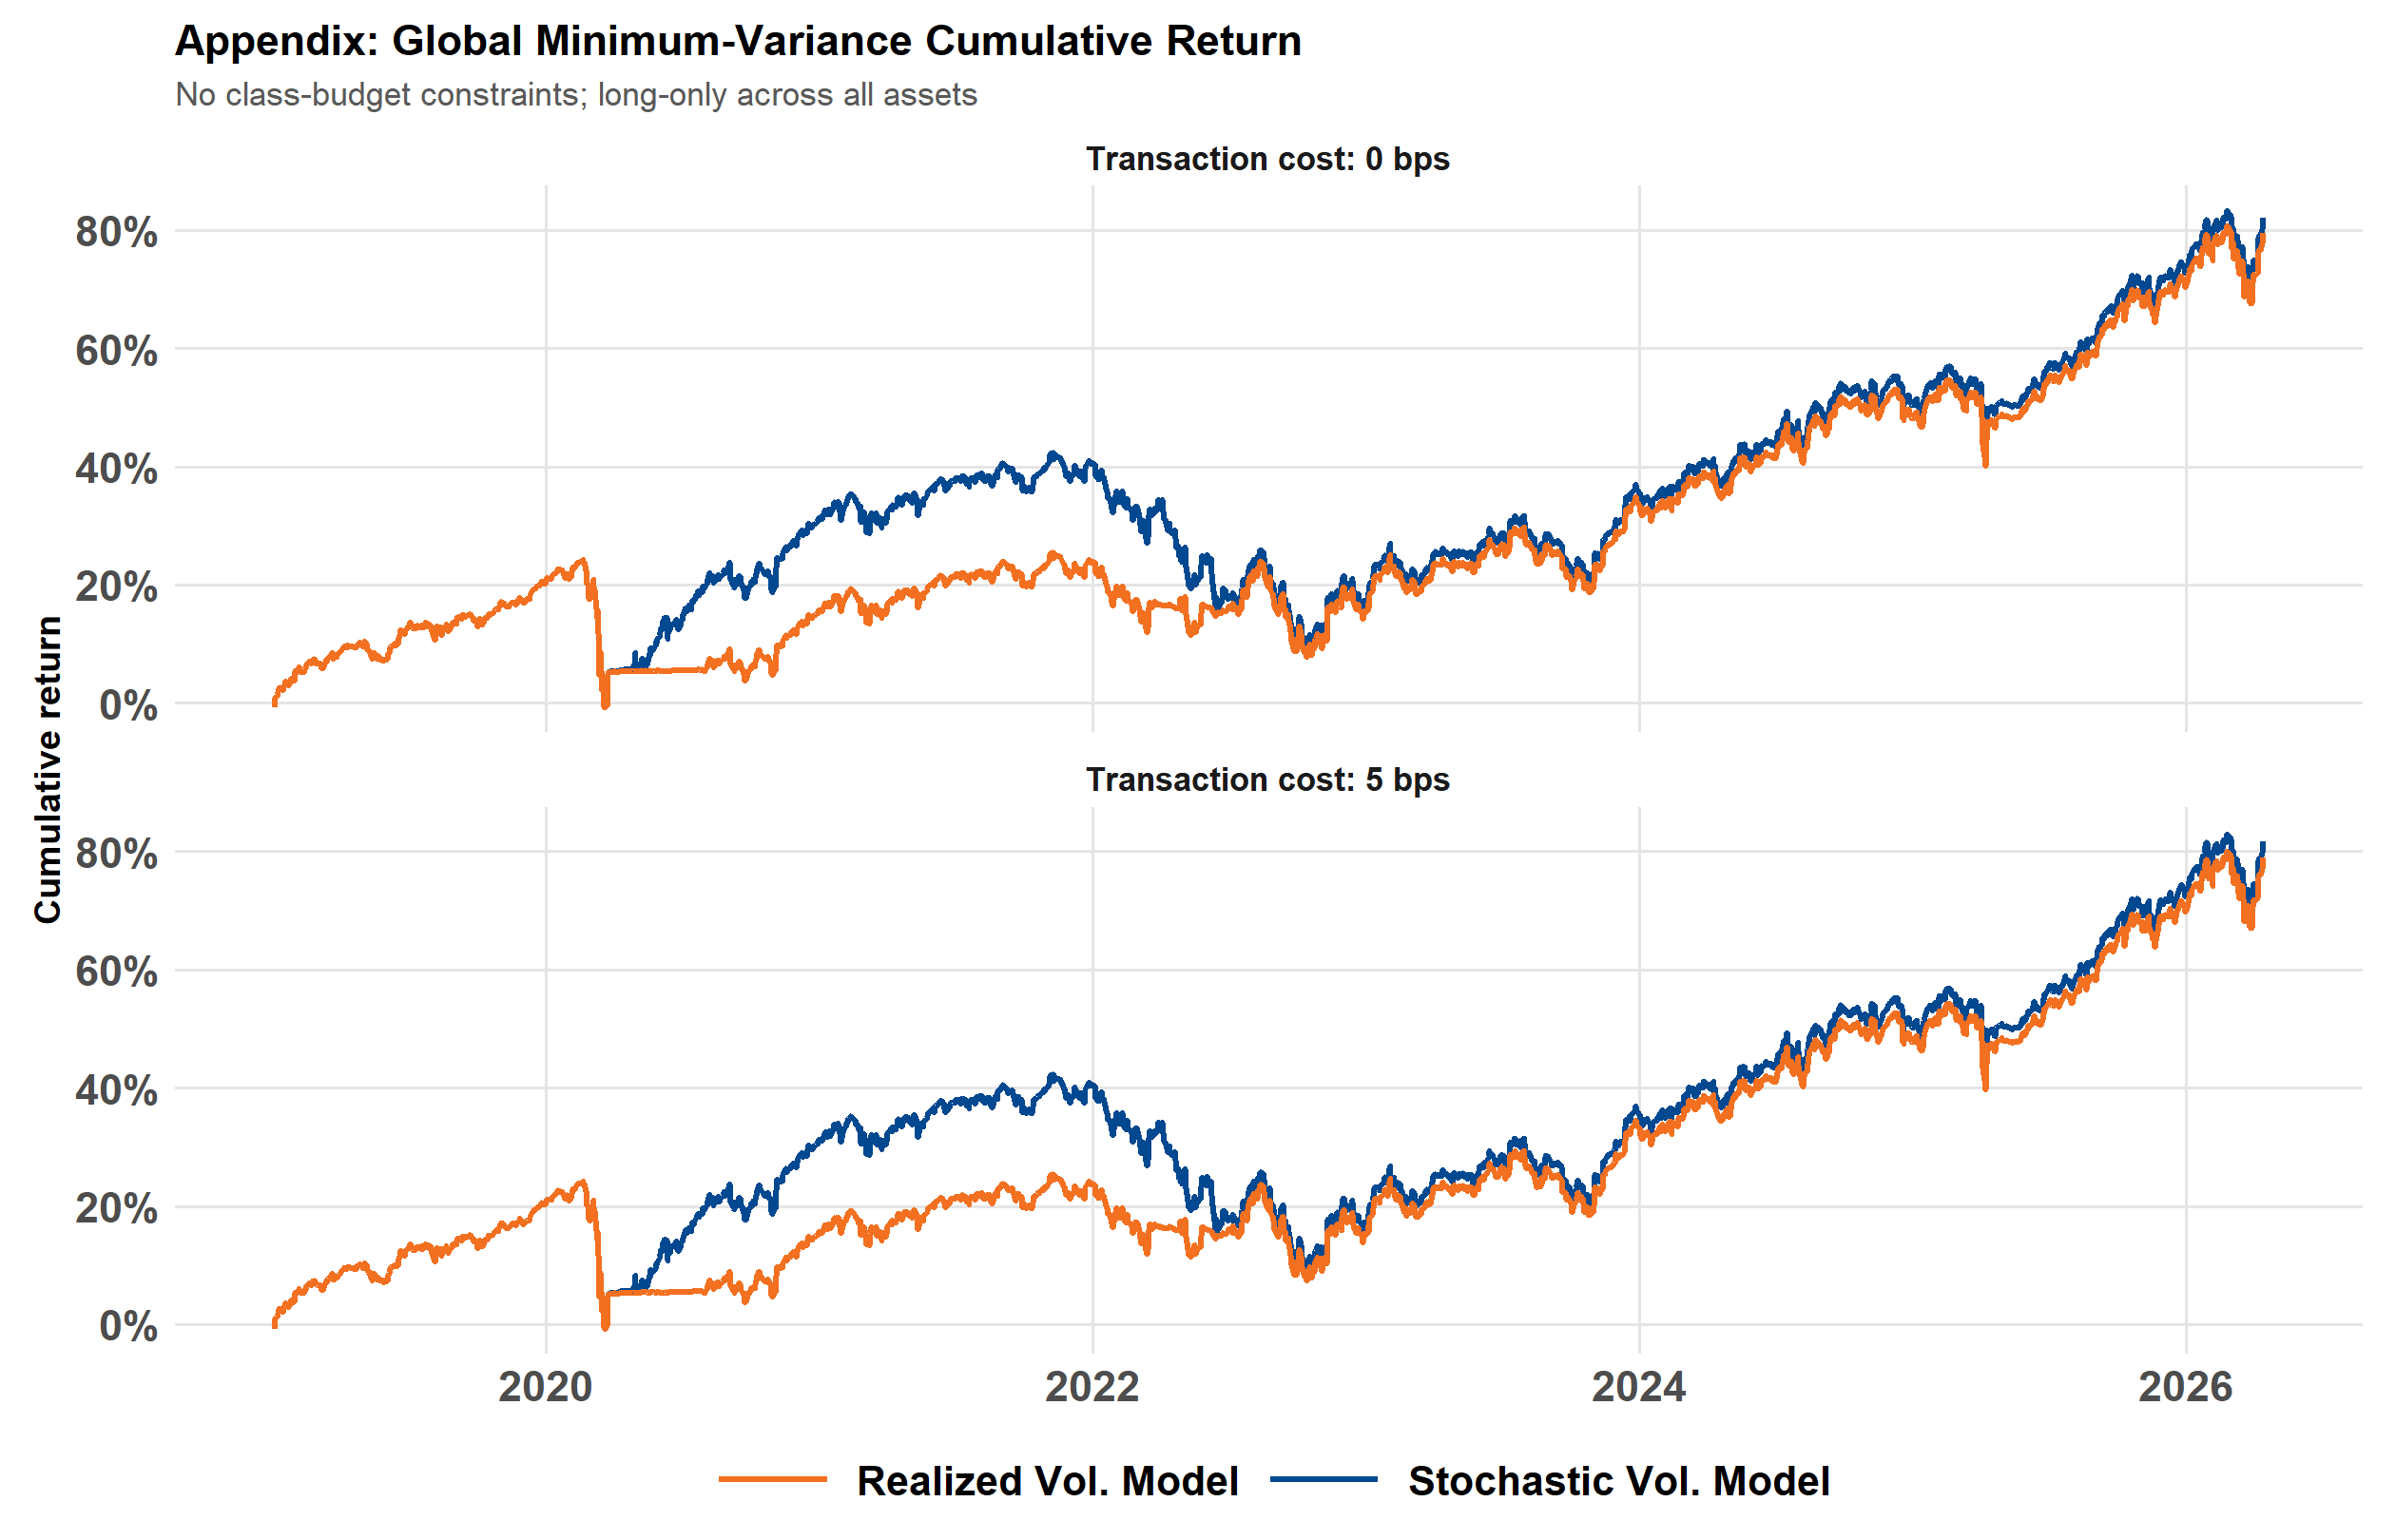
\includegraphics[width=0.92\textwidth]{../03_Results/Charts/appendix_minvar_cumulative_return.png}
    \caption{Global long-only minimum-variance portfolios (no class-budget constraints):
             realized-vol covariance vs.\ stochastic-vol covariance, shown for 0 and 5 bps costs.}
  \end{figure}

\end{frame}

%---- A.4 - Global Minimum-Variance: Rolling Return/Vol Ratio -----------------%

\begin{frame}{Appendix -- Global Minimum-Variance: Rolling Return/Volatility Ratio}

  \begin{figure}
    \centering
    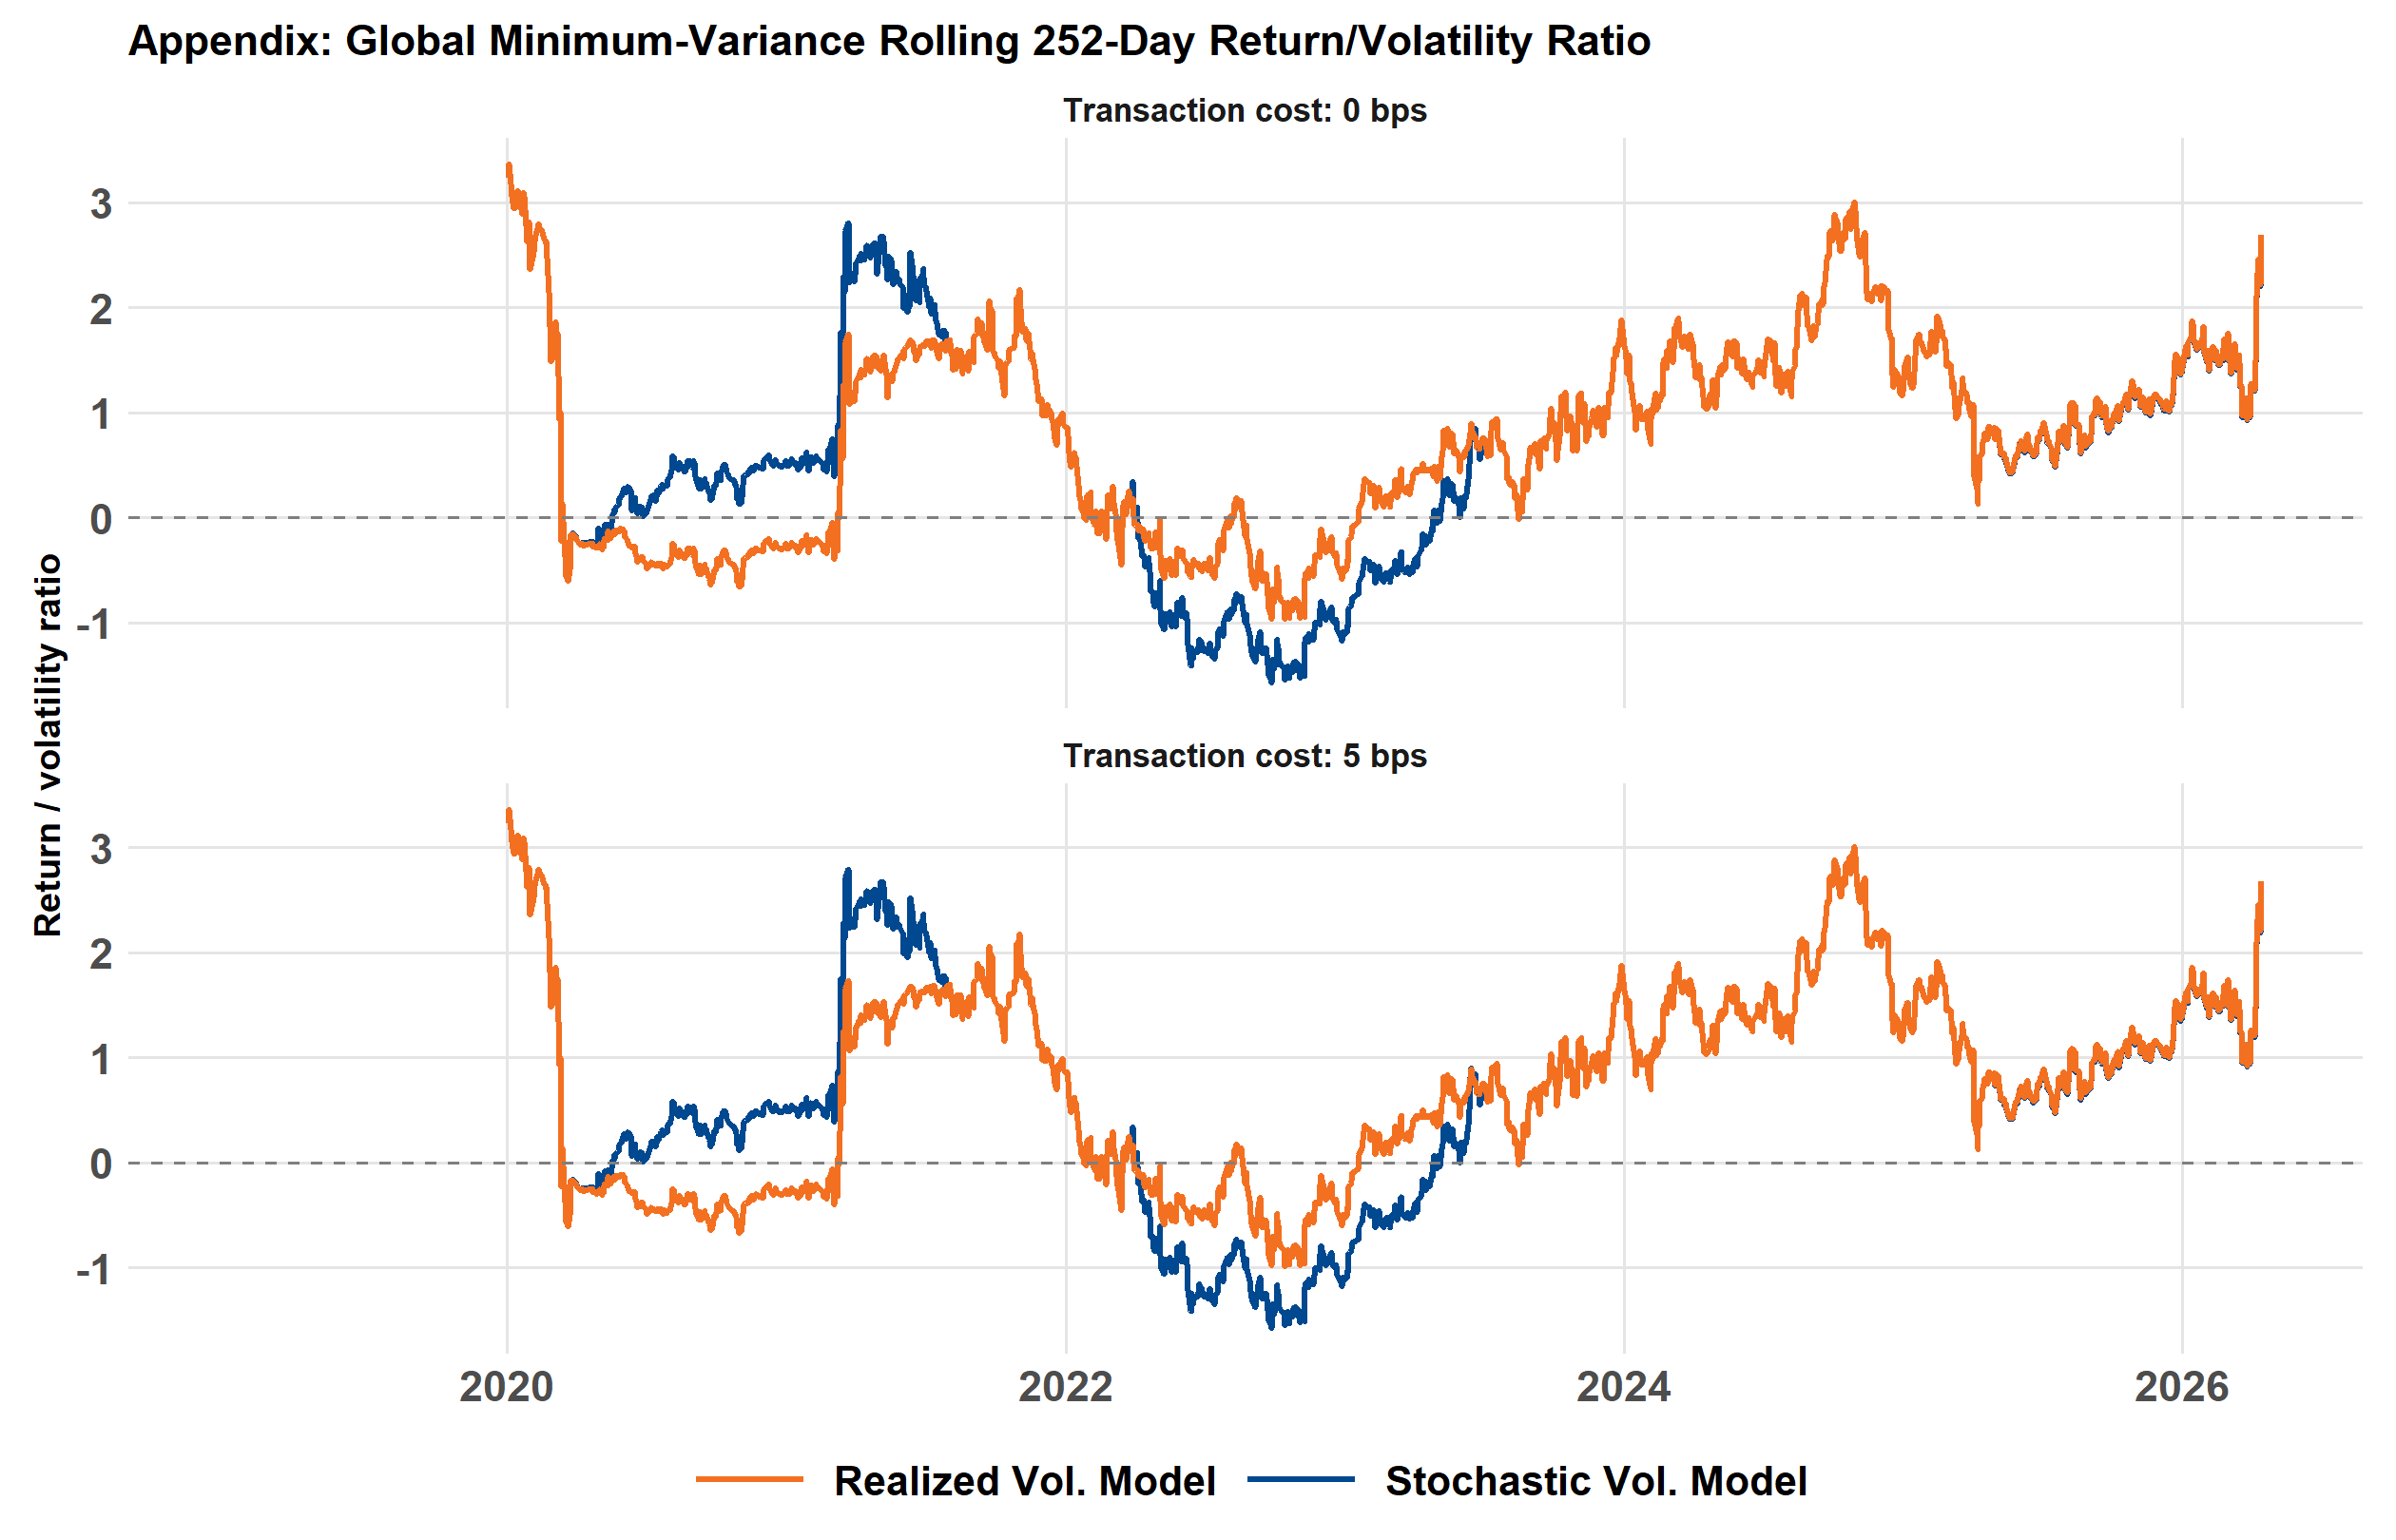
\includegraphics[width=0.92\textwidth]{../03_Results/Charts/appendix_minvar_rolling_252_ratio.png}
    \caption{Rolling 252-day return/volatility ratio for global minimum-variance portfolios,
             for 0 and 5 bps transaction costs.}
  \end{figure}

\end{frame}

%---- A.5 - Performance Metrics Tables ----------------------------------------%

\begin{frame}{Appendix -- Full Performance Metrics}

  \vspace{0.3em}
  {\footnotesize \textbf{Part 1: Single-Asset SPY (0 bps, Jan 2019 -- Dec 2024)}}

  \vspace{0.2em}
  {\footnotesize
  \begin{tabular}{@{}lrrrrrr@{}}
    \toprule
    & \textbf{SPY} & \textbf{Realized Vol.} & \textbf{FSV} \\
    \midrule
    Ann.\ Return     & 16.8\% & 5.3\%  & 7.1\% \\
    Ann.\ Vol        & 19.6\% & 15.2\% & 14.3\% \\
    Ret/Vol          & 0.859  & 0.352  & 0.496 \\
    Max Drawdown     & $-$33.7\% & $-$25.8\% & $-$27.7\% \\
    ES (5\%)         & $-$2.95\% & $-$2.60\% & $-$2.32\% \\
    Turnover (p.a.)  & 0.00 & 5.96 & 4.56 \\
    \bottomrule
  \end{tabular}
  }

  \vspace{0.6em}
  {\footnotesize \textbf{Part 2: Multi-Asset Budgets (0 bps)}}

  \vspace{0.2em}
  {\footnotesize
  \setlength{\tabcolsep}{4pt}
  \begin{tabular}{@{}llrrrrr@{}}
    \toprule
    \textbf{Portfolio} & \textbf{Strategy} & \textbf{Ret} & \textbf{Vol} & \textbf{R/V} & \textbf{MaxDD} & \textbf{Turn.} \\
    \midrule
    pf1 (45/45/10) & Realized Vol.\ Model & 11.5\% & 10.5\% & 1.097 & $-$21.9\% & 3.78 \\
    pf1 (45/45/10) & FSV                 & 12.3\% & 11.3\% & 1.089 & $-$20.9\% & 2.73 \\
    \midrule
    pf2 (60/40/0)  & Realized Vol.\ Model & 12.0\% & 12.8\% & 0.942 & $-$25.3\% & 4.54 \\
    pf2 (60/40/0)  & FSV                 & 12.9\% & 13.7\% & 0.939 & $-$23.5\% & 3.24 \\
    \bottomrule
  \end{tabular}
  }

\end{frame}

%---- A.6 - Asset Universe ----------------------------------------------------%

\begin{frame}{Appendix -- Asset Universe and Class Weights}

  {\scriptsize
  \setlength{\tabcolsep}{3pt}
  \begin{tabular}{@{}lllrcc@{}}
    \toprule
    \textbf{Ticker} & \textbf{Name} & \textbf{Class} & \textbf{Within-Class} & \textbf{pf1 Class} & \textbf{pf2 Class} \\
    \midrule
    SPY & SPDR S\&P 500 ETF Trust & Equity & 40\% & 45\% & 60\% \\
    QQQ & Invesco QQQ Trust & Equity & 20\% & 45\% & 60\% \\
    IWM & iShares Russell 2000 ETF & Equity & 20\% & 45\% & 60\% \\
    EFA & iShares MSCI EAFE ETF & Equity & 10\% & 45\% & 60\% \\
    EEM & iShares MSCI Emerging Markets ETF & Equity & 10\% & 45\% & 60\% \\
    \midrule
    TLT & iShares 20+ Year Treasury Bond ETF & Bonds & 30\% & 45\% & 40\% \\
    SHY & iShares 1--3 Year Treasury Bond ETF & Bonds & 30\% & 45\% & 40\% \\
    LQD & iShares iBoxx \$ Inv.\ Grade Corp.\ Bond ETF & Bonds & 25\% & 45\% & 40\% \\
    HYG & iShares iBoxx \$ High Yield Corp.\ Bond ETF & Bonds & 15\% & 45\% & 40\% \\
    \midrule
    GLD & SPDR Gold Shares & Gold & 100\% & 10\% & 0\% \\
    \bottomrule
  \end{tabular}
  }

  \vspace{0.4em}
  {\footnotesize Data source: Yahoo Finance via \texttt{quantmod::getSymbols()}, daily adjusted prices.}

\end{frame}

%---- A.8 - Local vs GCP Comparison (Part 1) ----------------------------------%

\begin{frame}{Appendix -- Local vs GCP Differences (Part 1)}
  {\scriptsize
  \setlength{\tabcolsep}{4pt}
  \begin{tabular}{@{}lrrrrr@{}}
    \toprule
    \textbf{Strategy} & \textbf{Return} & \textbf{Vol} & \textbf{Sharpe} & \textbf{Max DD} & \textbf{Turnover} \\
    \midrule
    SPY Benchmark       & 16.9\% & 19.6\% & 0.865 & $-$33.7\% & 0.00 \\
    Naive MM (Realized) & 5.4\%  & 15.1\% & 0.355 & $-$25.8\% & 5.95 \\
    FSV MM -- Local     & 7.1\%  & 14.3\% & 0.496 & $-$27.7\% & 4.56 \\
    FSV MM -- GCP       & 5.8\%  & 15.8\% & 0.365 & $-$31.0\% & 5.37 \\
    \bottomrule
  \end{tabular}
  }

  \vspace{0.5em}
  {\footnotesize Key difference: with deeper GCP convergence, FSV and Naive are nearly indistinguishable on Sharpe (0.365 vs 0.355).}
\end{frame}

%---- A.9 - Local vs GCP Comparison (Part 2) ----------------------------------%

\begin{frame}{Appendix -- Local vs GCP Differences (Part 2)}
  {\scriptsize
  \setlength{\tabcolsep}{4pt}
  \begin{tabular}{@{}lrrrrr@{}}
    \toprule
    \textbf{Strategy (pf1, 0 bps)} & \textbf{Return} & \textbf{Vol} & \textbf{Sharpe} & \textbf{Max DD} & \textbf{Turnover} \\
    \midrule
    Rolling MV -- Local & 11.5\% & 10.5\% & 1.097 & $-$21.9\% & 3.78 \\
    Rolling MV -- GCP   & 11.5\% & 10.5\% & 1.099 & $-$21.9\% & 3.78 \\
    FSV MV -- Local     & 12.3\% & 11.3\% & 1.089 & $-$20.9\% & 2.73 \\
    FSV MV -- GCP       & 12.1\% & 11.2\% & 1.079 & $-$21.6\% & 2.91 \\
    \bottomrule
  \end{tabular}
  }

  \vspace{0.5em}
  {\footnotesize Multi-asset conclusion is stable across compute settings; differences are small and mostly in the FSV leg.}
\end{frame}

%---- A.10 - Priors Used in FSV ----------------------------------------------%

\begin{frame}{Appendix -- FSV Priors Used}

  \vspace{0.2em}
  \begin{block}{Loadings Priors}
  {\scriptsize
  \texttt{priorfacloadtype="rowwiseng"}, \texttt{priorfacload=0.1}, \texttt{priorng=c(1,1)}:
  row-wise Normal-Gamma shrinkage, pulling small loadings toward zero while allowing large loadings when supported by data.}
  \end{block}

  \vspace{-0.2em}
  \begin{block}{SV AR(1) Priors}
  {\scriptsize
  \texttt{priormu=c(0,10)} (diffuse on $\mu$), \texttt{priorphiidi=priorphifac=c(10,3)} (persistent $\phi$, prior mean $10/13\approx0.77$),
  \texttt{priorsigmaidi=priorsigmafac=1} (Exponential(1) on vol-of-vol),
  and \texttt{priorh0idi=priorh0fac="stationary"} for initial states.}
  \end{block}

  \vspace{-0.2em}
  \begin{alertblock}{Key Implication in This Project}
  {\scriptsize
  Posterior persistence moved close to the upper clamp in many series (around 0.999), indicating that the data dominates the prior on $\phi$ and implies very strong volatility persistence, which is typical in financial return volatility.}
  \end{alertblock}

\end{frame}

%---- AI Disclaimer -----------------------------------------------------------%

\begin{frame}{AI Disclaimer}

  \begin{block}{AI-Assisted Tools Used}
    The following AI-assisted language and coding models were used in the
    preparation of this work:
    \textbf{Claude} (Sonnet 4.6 and Opus 4.6, Anthropic),
    \textbf{ChatGPT Codex} (OpenAI), and
    \textbf{Gemini} (Google).
  \end{block}

  \vspace{0.5em}

  \begin{itemize}
    \setlength\itemsep{0.7em}
    \item \textbf{Claude} and \textbf{ChatGPT Codex} were used to support the
          implementation of the analytical pipeline, including code generation and
          debugging, validation of model outputs, summarisation of results, and the
          production of charts and figures.
    \item \textbf{Gemini} was used to cross-validate selected results and to assist
          with spelling and language checking.
  \end{itemize}

  \vspace{0.5em}

  \begin{alertblock}{}
    \centering
    All AI-generated outputs were reviewed, critically assessed, and adapted by
    the authors.
  \end{alertblock}

\end{frame}

%==== END =====================================================================%

\end{document}
